\begin{figure}[H] \centering % Created by tikzDevice version 0.12.4 on 2023-08-13 18:28:58
% !TEX encoding = UTF-8 Unicode
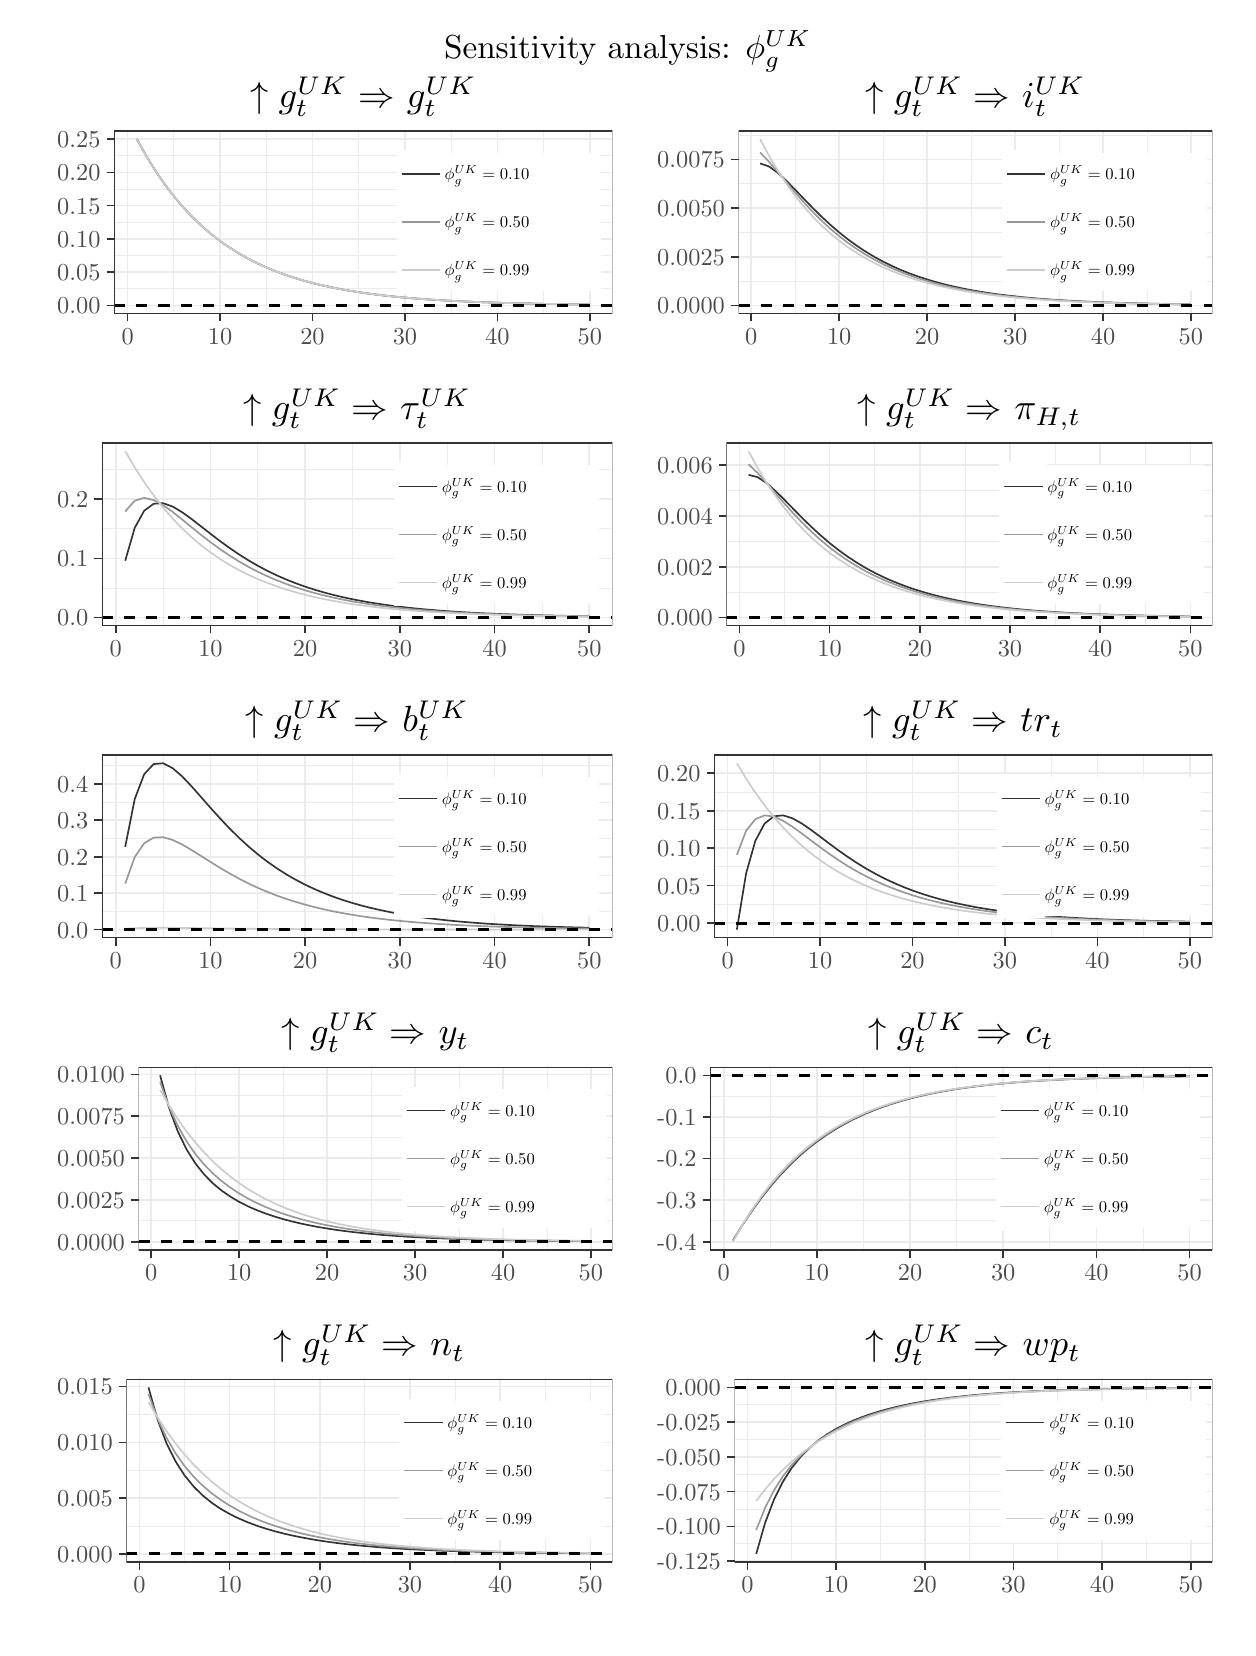
\begin{tikzpicture}[x=1pt,y=1pt]
\definecolor{fillColor}{RGB}{255,255,255}
\path[use as bounding box,fill=fillColor,fill opacity=0.00] (0,0) rectangle (433.62,578.16);
\begin{scope}
\path[clip] (  0.00,451.10) rectangle (216.81,563.87);
\definecolor{drawColor}{RGB}{255,255,255}
\definecolor{fillColor}{RGB}{255,255,255}

\path[draw=drawColor,line width= 0.6pt,line join=round,line cap=round,fill=fillColor] (  0.00,451.10) rectangle (216.81,563.87);
\end{scope}
\begin{scope}
\path[clip] ( 31.27,474.78) rectangle (211.31,540.91);
\definecolor{fillColor}{RGB}{255,255,255}

\path[fill=fillColor] ( 31.27,474.78) rectangle (211.31,540.91);
\definecolor{drawColor}{gray}{0.92}

\path[draw=drawColor,line width= 0.3pt,line join=round] ( 31.27,483.79) --
	(211.31,483.79);

\path[draw=drawColor,line width= 0.3pt,line join=round] ( 31.27,495.82) --
	(211.31,495.82);

\path[draw=drawColor,line width= 0.3pt,line join=round] ( 31.27,507.84) --
	(211.31,507.84);

\path[draw=drawColor,line width= 0.3pt,line join=round] ( 31.27,519.87) --
	(211.31,519.87);

\path[draw=drawColor,line width= 0.3pt,line join=round] ( 31.27,531.89) --
	(211.31,531.89);

\path[draw=drawColor,line width= 0.3pt,line join=round] ( 52.81,474.78) --
	( 52.81,540.91);

\path[draw=drawColor,line width= 0.3pt,line join=round] ( 86.22,474.78) --
	( 86.22,540.91);

\path[draw=drawColor,line width= 0.3pt,line join=round] (119.62,474.78) --
	(119.62,540.91);

\path[draw=drawColor,line width= 0.3pt,line join=round] (153.02,474.78) --
	(153.02,540.91);

\path[draw=drawColor,line width= 0.3pt,line join=round] (186.43,474.78) --
	(186.43,540.91);

\path[draw=drawColor,line width= 0.6pt,line join=round] ( 31.27,477.78) --
	(211.31,477.78);

\path[draw=drawColor,line width= 0.6pt,line join=round] ( 31.27,489.81) --
	(211.31,489.81);

\path[draw=drawColor,line width= 0.6pt,line join=round] ( 31.27,501.83) --
	(211.31,501.83);

\path[draw=drawColor,line width= 0.6pt,line join=round] ( 31.27,513.86) --
	(211.31,513.86);

\path[draw=drawColor,line width= 0.6pt,line join=round] ( 31.27,525.88) --
	(211.31,525.88);

\path[draw=drawColor,line width= 0.6pt,line join=round] ( 31.27,537.90) --
	(211.31,537.90);

\path[draw=drawColor,line width= 0.6pt,line join=round] ( 36.11,474.78) --
	( 36.11,540.91);

\path[draw=drawColor,line width= 0.6pt,line join=round] ( 69.52,474.78) --
	( 69.52,540.91);

\path[draw=drawColor,line width= 0.6pt,line join=round] (102.92,474.78) --
	(102.92,540.91);

\path[draw=drawColor,line width= 0.6pt,line join=round] (136.32,474.78) --
	(136.32,540.91);

\path[draw=drawColor,line width= 0.6pt,line join=round] (169.72,474.78) --
	(169.72,540.91);

\path[draw=drawColor,line width= 0.6pt,line join=round] (203.13,474.78) --
	(203.13,540.91);
\definecolor{drawColor}{gray}{0.20}

\path[draw=drawColor,line width= 0.6pt,line join=round] ( 39.45,537.90) --
	( 42.79,531.89) --
	( 46.13,526.48) --
	( 49.47,521.61) --
	( 52.81,517.23) --
	( 56.15,513.28) --
	( 59.50,509.73) --
	( 62.84,506.54) --
	( 66.18,503.66) --
	( 69.52,501.07) --
	( 72.86,498.75) --
	( 76.20,496.65) --
	( 79.54,494.76) --
	( 82.88,493.06) --
	( 86.22,491.54) --
	( 89.56,490.16) --
	( 92.90,488.92) --
	( 96.24,487.81) --
	( 99.58,486.81) --
	(102.92,485.90) --
	(106.26,485.09) --
	(109.60,484.36) --
	(112.94,483.70) --
	(116.28,483.11) --
	(119.62,482.58) --
	(122.96,482.10) --
	(126.30,481.67) --
	(129.64,481.28) --
	(132.98,480.93) --
	(136.32,480.61) --
	(139.66,480.33) --
	(143.00,480.08) --
	(146.34,479.85) --
	(149.68,479.64) --
	(153.02,479.45) --
	(156.36,479.29) --
	(159.70,479.14) --
	(163.04,479.00) --
	(166.38,478.88) --
	(169.72,478.77) --
	(173.06,478.67) --
	(176.40,478.58) --
	(179.74,478.50) --
	(183.08,478.43) --
	(186.43,478.36) --
	(189.77,478.31) --
	(193.11,478.25) --
	(196.45,478.21) --
	(199.79,478.16) --
	(203.13,478.13);
\definecolor{drawColor}{RGB}{152,152,152}

\path[draw=drawColor,line width= 0.6pt,line join=round] ( 39.45,537.90) --
	( 42.79,531.89) --
	( 46.13,526.48) --
	( 49.47,521.61) --
	( 52.81,517.23) --
	( 56.15,513.28) --
	( 59.50,509.73) --
	( 62.84,506.54) --
	( 66.18,503.66) --
	( 69.52,501.07) --
	( 72.86,498.75) --
	( 76.20,496.65) --
	( 79.54,494.76) --
	( 82.88,493.06) --
	( 86.22,491.54) --
	( 89.56,490.16) --
	( 92.90,488.92) --
	( 96.24,487.81) --
	( 99.58,486.81) --
	(102.92,485.90) --
	(106.26,485.09) --
	(109.60,484.36) --
	(112.94,483.70) --
	(116.28,483.11) --
	(119.62,482.58) --
	(122.96,482.10) --
	(126.30,481.67) --
	(129.64,481.28) --
	(132.98,480.93) --
	(136.32,480.61) --
	(139.66,480.33) --
	(143.00,480.08) --
	(146.34,479.85) --
	(149.68,479.64) --
	(153.02,479.45) --
	(156.36,479.29) --
	(159.70,479.14) --
	(163.04,479.00) --
	(166.38,478.88) --
	(169.72,478.77) --
	(173.06,478.67) --
	(176.40,478.58) --
	(179.74,478.50) --
	(183.08,478.43) --
	(186.43,478.36) --
	(189.77,478.31) --
	(193.11,478.25) --
	(196.45,478.21) --
	(199.79,478.16) --
	(203.13,478.13);
\definecolor{drawColor}{gray}{0.80}

\path[draw=drawColor,line width= 0.6pt,line join=round] ( 39.45,537.90) --
	( 42.79,531.89) --
	( 46.13,526.48) --
	( 49.47,521.61) --
	( 52.81,517.23) --
	( 56.15,513.28) --
	( 59.50,509.73) --
	( 62.84,506.54) --
	( 66.18,503.66) --
	( 69.52,501.07) --
	( 72.86,498.75) --
	( 76.20,496.65) --
	( 79.54,494.76) --
	( 82.88,493.06) --
	( 86.22,491.54) --
	( 89.56,490.16) --
	( 92.90,488.92) --
	( 96.24,487.81) --
	( 99.58,486.81) --
	(102.92,485.90) --
	(106.26,485.09) --
	(109.60,484.36) --
	(112.94,483.70) --
	(116.28,483.11) --
	(119.62,482.58) --
	(122.96,482.10) --
	(126.30,481.67) --
	(129.64,481.28) --
	(132.98,480.93) --
	(136.32,480.61) --
	(139.66,480.33) --
	(143.00,480.08) --
	(146.34,479.85) --
	(149.68,479.64) --
	(153.02,479.45) --
	(156.36,479.29) --
	(159.70,479.14) --
	(163.04,479.00) --
	(166.38,478.88) --
	(169.72,478.77) --
	(173.06,478.67) --
	(176.40,478.58) --
	(179.74,478.50) --
	(183.08,478.43) --
	(186.43,478.36) --
	(189.77,478.31) --
	(193.11,478.25) --
	(196.45,478.21) --
	(199.79,478.16) --
	(203.13,478.13);
\definecolor{drawColor}{RGB}{0,0,0}

\path[draw=drawColor,line width= 1.1pt,dash pattern=on 4pt off 4pt ,line join=round] ( 31.27,477.78) -- (211.31,477.78);
\definecolor{drawColor}{gray}{0.20}

\path[draw=drawColor,line width= 0.6pt,line join=round,line cap=round] ( 31.27,474.78) rectangle (211.31,540.91);
\end{scope}
\begin{scope}
\path[clip] (  0.00,  0.00) rectangle (433.62,578.16);
\definecolor{drawColor}{gray}{0.30}

\node[text=drawColor,anchor=base east,inner sep=0pt, outer sep=0pt, scale=  0.88] at ( 26.32,474.75) {0.00};

\node[text=drawColor,anchor=base east,inner sep=0pt, outer sep=0pt, scale=  0.88] at ( 26.32,486.78) {0.05};

\node[text=drawColor,anchor=base east,inner sep=0pt, outer sep=0pt, scale=  0.88] at ( 26.32,498.80) {0.10};

\node[text=drawColor,anchor=base east,inner sep=0pt, outer sep=0pt, scale=  0.88] at ( 26.32,510.83) {0.15};

\node[text=drawColor,anchor=base east,inner sep=0pt, outer sep=0pt, scale=  0.88] at ( 26.32,522.85) {0.20};

\node[text=drawColor,anchor=base east,inner sep=0pt, outer sep=0pt, scale=  0.88] at ( 26.32,534.87) {0.25};
\end{scope}
\begin{scope}
\path[clip] (  0.00,  0.00) rectangle (433.62,578.16);
\definecolor{drawColor}{gray}{0.20}

\path[draw=drawColor,line width= 0.6pt,line join=round] ( 28.52,477.78) --
	( 31.27,477.78);

\path[draw=drawColor,line width= 0.6pt,line join=round] ( 28.52,489.81) --
	( 31.27,489.81);

\path[draw=drawColor,line width= 0.6pt,line join=round] ( 28.52,501.83) --
	( 31.27,501.83);

\path[draw=drawColor,line width= 0.6pt,line join=round] ( 28.52,513.86) --
	( 31.27,513.86);

\path[draw=drawColor,line width= 0.6pt,line join=round] ( 28.52,525.88) --
	( 31.27,525.88);

\path[draw=drawColor,line width= 0.6pt,line join=round] ( 28.52,537.90) --
	( 31.27,537.90);
\end{scope}
\begin{scope}
\path[clip] (  0.00,  0.00) rectangle (433.62,578.16);
\definecolor{drawColor}{gray}{0.20}

\path[draw=drawColor,line width= 0.6pt,line join=round] ( 36.11,472.03) --
	( 36.11,474.78);

\path[draw=drawColor,line width= 0.6pt,line join=round] ( 69.52,472.03) --
	( 69.52,474.78);

\path[draw=drawColor,line width= 0.6pt,line join=round] (102.92,472.03) --
	(102.92,474.78);

\path[draw=drawColor,line width= 0.6pt,line join=round] (136.32,472.03) --
	(136.32,474.78);

\path[draw=drawColor,line width= 0.6pt,line join=round] (169.72,472.03) --
	(169.72,474.78);

\path[draw=drawColor,line width= 0.6pt,line join=round] (203.13,472.03) --
	(203.13,474.78);
\end{scope}
\begin{scope}
\path[clip] (  0.00,  0.00) rectangle (433.62,578.16);
\definecolor{drawColor}{gray}{0.30}

\node[text=drawColor,anchor=base,inner sep=0pt, outer sep=0pt, scale=  0.88] at ( 36.11,463.76) {0};

\node[text=drawColor,anchor=base,inner sep=0pt, outer sep=0pt, scale=  0.88] at ( 69.52,463.76) {10};

\node[text=drawColor,anchor=base,inner sep=0pt, outer sep=0pt, scale=  0.88] at (102.92,463.76) {20};

\node[text=drawColor,anchor=base,inner sep=0pt, outer sep=0pt, scale=  0.88] at (136.32,463.76) {30};

\node[text=drawColor,anchor=base,inner sep=0pt, outer sep=0pt, scale=  0.88] at (169.72,463.76) {40};

\node[text=drawColor,anchor=base,inner sep=0pt, outer sep=0pt, scale=  0.88] at (203.13,463.76) {50};
\end{scope}
\begin{scope}
\path[clip] (  0.00,  0.00) rectangle (433.62,578.16);
\definecolor{fillColor}{RGB}{255,255,255}

\path[fill=fillColor] (134.34,482.83) rectangle (207.26,532.86);
\end{scope}
\begin{scope}
\path[clip] (  0.00,  0.00) rectangle (433.62,578.16);
\definecolor{fillColor}{RGB}{255,255,255}

\path[fill=fillColor] (133.34,516.52) rectangle (150.69,533.86);
\end{scope}
\begin{scope}
\path[clip] (  0.00,  0.00) rectangle (433.62,578.16);
\definecolor{drawColor}{gray}{0.20}

\path[draw=drawColor,line width= 0.6pt,line join=round] (135.08,525.19) -- (148.95,525.19);
\end{scope}
\begin{scope}
\path[clip] (  0.00,  0.00) rectangle (433.62,578.16);
\definecolor{drawColor}{gray}{0.20}

\path[draw=drawColor,line width= 0.6pt,line join=round] (135.08,525.19) -- (148.95,525.19);
\end{scope}
\begin{scope}
\path[clip] (  0.00,  0.00) rectangle (433.62,578.16);
\definecolor{drawColor}{gray}{0.20}

\path[draw=drawColor,line width= 0.6pt,line join=round] (135.08,525.19) -- (148.95,525.19);
\end{scope}
\begin{scope}
\path[clip] (  0.00,  0.00) rectangle (433.62,578.16);
\definecolor{fillColor}{RGB}{255,255,255}

\path[fill=fillColor] (133.34,499.17) rectangle (150.69,516.52);
\end{scope}
\begin{scope}
\path[clip] (  0.00,  0.00) rectangle (433.62,578.16);
\definecolor{drawColor}{RGB}{152,152,152}

\path[draw=drawColor,line width= 0.6pt,line join=round] (135.08,507.84) -- (148.95,507.84);
\end{scope}
\begin{scope}
\path[clip] (  0.00,  0.00) rectangle (433.62,578.16);
\definecolor{drawColor}{RGB}{152,152,152}

\path[draw=drawColor,line width= 0.6pt,line join=round] (135.08,507.84) -- (148.95,507.84);
\end{scope}
\begin{scope}
\path[clip] (  0.00,  0.00) rectangle (433.62,578.16);
\definecolor{drawColor}{RGB}{152,152,152}

\path[draw=drawColor,line width= 0.6pt,line join=round] (135.08,507.84) -- (148.95,507.84);
\end{scope}
\begin{scope}
\path[clip] (  0.00,  0.00) rectangle (433.62,578.16);
\definecolor{fillColor}{RGB}{255,255,255}

\path[fill=fillColor] (133.34,481.83) rectangle (150.69,499.17);
\end{scope}
\begin{scope}
\path[clip] (  0.00,  0.00) rectangle (433.62,578.16);
\definecolor{drawColor}{gray}{0.80}

\path[draw=drawColor,line width= 0.6pt,line join=round] (135.08,490.50) -- (148.95,490.50);
\end{scope}
\begin{scope}
\path[clip] (  0.00,  0.00) rectangle (433.62,578.16);
\definecolor{drawColor}{gray}{0.80}

\path[draw=drawColor,line width= 0.6pt,line join=round] (135.08,490.50) -- (148.95,490.50);
\end{scope}
\begin{scope}
\path[clip] (  0.00,  0.00) rectangle (433.62,578.16);
\definecolor{drawColor}{gray}{0.80}

\path[draw=drawColor,line width= 0.6pt,line join=round] (135.08,490.50) -- (148.95,490.50);
\end{scope}
\begin{scope}
\path[clip] (  0.00,  0.00) rectangle (433.62,578.16);
\definecolor{drawColor}{RGB}{0,0,0}

\node[text=drawColor,anchor=base west,inner sep=0pt, outer sep=0pt, scale=  0.60] at (150.69,523.12) {${\phi_g^{UK}}=0.10$};
\end{scope}
\begin{scope}
\path[clip] (  0.00,  0.00) rectangle (433.62,578.16);
\definecolor{drawColor}{RGB}{0,0,0}

\node[text=drawColor,anchor=base west,inner sep=0pt, outer sep=0pt, scale=  0.60] at (150.69,505.78) {${\phi_g^{UK}}=0.50$};
\end{scope}
\begin{scope}
\path[clip] (  0.00,  0.00) rectangle (433.62,578.16);
\definecolor{drawColor}{RGB}{0,0,0}

\node[text=drawColor,anchor=base west,inner sep=0pt, outer sep=0pt, scale=  0.60] at (150.69,488.43) {${\phi_g^{UK}}=0.99$};
\end{scope}
\begin{scope}
\path[clip] (  0.00,  0.00) rectangle (433.62,578.16);
\definecolor{drawColor}{RGB}{0,0,0}

\node[text=drawColor,anchor=base,inner sep=0pt, outer sep=0pt, scale=  1.32] at (121.29,549.28) {$\uparrow  g^{UK}_t \Rightarrow $ ${g^{UK}_t}$};
\end{scope}
\begin{scope}
\path[clip] (216.81,451.10) rectangle (433.62,563.87);
\definecolor{drawColor}{RGB}{255,255,255}
\definecolor{fillColor}{RGB}{255,255,255}

\path[draw=drawColor,line width= 0.6pt,line join=round,line cap=round,fill=fillColor] (216.81,451.10) rectangle (433.62,563.87);
\end{scope}
\begin{scope}
\path[clip] (256.88,474.78) rectangle (428.12,540.91);
\definecolor{fillColor}{RGB}{255,255,255}

\path[fill=fillColor] (256.88,474.78) rectangle (428.12,540.91);
\definecolor{drawColor}{gray}{0.92}

\path[draw=drawColor,line width= 0.3pt,line join=round] (256.88,486.57) --
	(428.12,486.57);

\path[draw=drawColor,line width= 0.3pt,line join=round] (256.88,504.14) --
	(428.12,504.14);

\path[draw=drawColor,line width= 0.3pt,line join=round] (256.88,521.71) --
	(428.12,521.71);

\path[draw=drawColor,line width= 0.3pt,line join=round] (256.88,539.27) --
	(428.12,539.27);

\path[draw=drawColor,line width= 0.3pt,line join=round] (277.37,474.78) --
	(277.37,540.91);

\path[draw=drawColor,line width= 0.3pt,line join=round] (309.14,474.78) --
	(309.14,540.91);

\path[draw=drawColor,line width= 0.3pt,line join=round] (340.91,474.78) --
	(340.91,540.91);

\path[draw=drawColor,line width= 0.3pt,line join=round] (372.68,474.78) --
	(372.68,540.91);

\path[draw=drawColor,line width= 0.3pt,line join=round] (404.45,474.78) --
	(404.45,540.91);

\path[draw=drawColor,line width= 0.6pt,line join=round] (256.88,477.78) --
	(428.12,477.78);

\path[draw=drawColor,line width= 0.6pt,line join=round] (256.88,495.35) --
	(428.12,495.35);

\path[draw=drawColor,line width= 0.6pt,line join=round] (256.88,512.92) --
	(428.12,512.92);

\path[draw=drawColor,line width= 0.6pt,line join=round] (256.88,530.49) --
	(428.12,530.49);

\path[draw=drawColor,line width= 0.6pt,line join=round] (261.48,474.78) --
	(261.48,540.91);

\path[draw=drawColor,line width= 0.6pt,line join=round] (293.25,474.78) --
	(293.25,540.91);

\path[draw=drawColor,line width= 0.6pt,line join=round] (325.03,474.78) --
	(325.03,540.91);

\path[draw=drawColor,line width= 0.6pt,line join=round] (356.80,474.78) --
	(356.80,540.91);

\path[draw=drawColor,line width= 0.6pt,line join=round] (388.57,474.78) --
	(388.57,540.91);

\path[draw=drawColor,line width= 0.6pt,line join=round] (420.34,474.78) --
	(420.34,540.91);
\definecolor{drawColor}{gray}{0.20}

\path[draw=drawColor,line width= 0.6pt,line join=round] (264.66,529.08) --
	(267.84,528.02) --
	(271.02,525.74) --
	(274.19,522.81) --
	(277.37,519.56) --
	(280.55,516.24) --
	(283.72,512.97) --
	(286.90,509.84) --
	(290.08,506.90) --
	(293.25,504.17) --
	(296.43,501.65) --
	(299.61,499.34) --
	(302.79,497.24) --
	(305.96,495.33) --
	(309.14,493.60) --
	(312.32,492.04) --
	(315.49,490.62) --
	(318.67,489.35) --
	(321.85,488.20) --
	(325.03,487.16) --
	(328.20,486.22) --
	(331.38,485.38) --
	(334.56,484.62) --
	(337.73,483.94) --
	(340.91,483.32) --
	(344.09,482.77) --
	(347.26,482.27) --
	(350.44,481.82) --
	(353.62,481.42) --
	(356.80,481.06) --
	(359.97,480.73) --
	(363.15,480.43) --
	(366.33,480.17) --
	(369.50,479.93) --
	(372.68,479.71) --
	(375.86,479.52) --
	(379.03,479.35) --
	(382.21,479.19) --
	(385.39,479.05) --
	(388.57,478.92) --
	(391.74,478.81) --
	(394.92,478.71) --
	(398.10,478.61) --
	(401.27,478.53) --
	(404.45,478.46) --
	(407.63,478.39) --
	(410.81,478.33) --
	(413.98,478.27) --
	(417.16,478.22) --
	(420.34,478.18);
\definecolor{drawColor}{RGB}{152,152,152}

\path[draw=drawColor,line width= 0.6pt,line join=round] (264.66,533.05) --
	(267.84,529.78) --
	(271.02,526.11) --
	(274.19,522.31) --
	(277.37,518.55) --
	(280.55,514.95) --
	(283.72,511.55) --
	(286.90,508.39) --
	(290.08,505.48) --
	(293.25,502.81) --
	(296.43,500.37) --
	(299.61,498.16) --
	(302.79,496.15) --
	(305.96,494.34) --
	(309.14,492.70) --
	(312.32,491.21) --
	(315.49,489.88) --
	(318.67,488.67) --
	(321.85,487.59) --
	(325.03,486.61) --
	(328.20,485.73) --
	(331.38,484.93) --
	(334.56,484.22) --
	(337.73,483.57) --
	(340.91,483.00) --
	(344.09,482.47) --
	(347.26,482.01) --
	(350.44,481.58) --
	(353.62,481.20) --
	(356.80,480.86) --
	(359.97,480.55) --
	(363.15,480.28) --
	(366.33,480.03) --
	(369.50,479.80) --
	(372.68,479.60) --
	(375.86,479.42) --
	(379.03,479.25) --
	(382.21,479.11) --
	(385.39,478.97) --
	(388.57,478.86) --
	(391.74,478.75) --
	(394.92,478.65) --
	(398.10,478.56) --
	(401.27,478.49) --
	(404.45,478.42) --
	(407.63,478.35) --
	(410.81,478.30) --
	(413.98,478.24) --
	(417.16,478.20) --
	(420.34,478.16);
\definecolor{drawColor}{gray}{0.80}

\path[draw=drawColor,line width= 0.6pt,line join=round] (264.66,537.90) --
	(267.84,531.94) --
	(271.02,526.55) --
	(274.19,521.70) --
	(277.37,517.32) --
	(280.55,513.37) --
	(283.72,509.82) --
	(286.90,506.62) --
	(290.08,503.74) --
	(293.25,501.15) --
	(296.43,498.81) --
	(299.61,496.71) --
	(302.79,494.82) --
	(305.96,493.11) --
	(309.14,491.58) --
	(312.32,490.20) --
	(315.49,488.96) --
	(318.67,487.84) --
	(321.85,486.84) --
	(325.03,485.93) --
	(328.20,485.12) --
	(331.38,484.38) --
	(334.56,483.72) --
	(337.73,483.13) --
	(340.91,482.59) --
	(344.09,482.11) --
	(347.26,481.68) --
	(350.44,481.29) --
	(353.62,480.94) --
	(356.80,480.62) --
	(359.97,480.34) --
	(363.15,480.08) --
	(366.33,479.85) --
	(369.50,479.65) --
	(372.68,479.46) --
	(375.86,479.29) --
	(379.03,479.14) --
	(382.21,479.00) --
	(385.39,478.88) --
	(388.57,478.77) --
	(391.74,478.67) --
	(394.92,478.58) --
	(398.10,478.50) --
	(401.27,478.43) --
	(404.45,478.37) --
	(407.63,478.31) --
	(410.81,478.26) --
	(413.98,478.21) --
	(417.16,478.17) --
	(420.34,478.13);
\definecolor{drawColor}{RGB}{0,0,0}

\path[draw=drawColor,line width= 1.1pt,dash pattern=on 4pt off 4pt ,line join=round] (256.88,477.78) -- (428.12,477.78);
\definecolor{drawColor}{gray}{0.20}

\path[draw=drawColor,line width= 0.6pt,line join=round,line cap=round] (256.88,474.78) rectangle (428.12,540.91);
\end{scope}
\begin{scope}
\path[clip] (  0.00,  0.00) rectangle (433.62,578.16);
\definecolor{drawColor}{gray}{0.30}

\node[text=drawColor,anchor=base east,inner sep=0pt, outer sep=0pt, scale=  0.88] at (251.93,474.75) {0.0000};

\node[text=drawColor,anchor=base east,inner sep=0pt, outer sep=0pt, scale=  0.88] at (251.93,492.32) {0.0025};

\node[text=drawColor,anchor=base east,inner sep=0pt, outer sep=0pt, scale=  0.88] at (251.93,509.89) {0.0050};

\node[text=drawColor,anchor=base east,inner sep=0pt, outer sep=0pt, scale=  0.88] at (251.93,527.46) {0.0075};
\end{scope}
\begin{scope}
\path[clip] (  0.00,  0.00) rectangle (433.62,578.16);
\definecolor{drawColor}{gray}{0.20}

\path[draw=drawColor,line width= 0.6pt,line join=round] (254.13,477.78) --
	(256.88,477.78);

\path[draw=drawColor,line width= 0.6pt,line join=round] (254.13,495.35) --
	(256.88,495.35);

\path[draw=drawColor,line width= 0.6pt,line join=round] (254.13,512.92) --
	(256.88,512.92);

\path[draw=drawColor,line width= 0.6pt,line join=round] (254.13,530.49) --
	(256.88,530.49);
\end{scope}
\begin{scope}
\path[clip] (  0.00,  0.00) rectangle (433.62,578.16);
\definecolor{drawColor}{gray}{0.20}

\path[draw=drawColor,line width= 0.6pt,line join=round] (261.48,472.03) --
	(261.48,474.78);

\path[draw=drawColor,line width= 0.6pt,line join=round] (293.25,472.03) --
	(293.25,474.78);

\path[draw=drawColor,line width= 0.6pt,line join=round] (325.03,472.03) --
	(325.03,474.78);

\path[draw=drawColor,line width= 0.6pt,line join=round] (356.80,472.03) --
	(356.80,474.78);

\path[draw=drawColor,line width= 0.6pt,line join=round] (388.57,472.03) --
	(388.57,474.78);

\path[draw=drawColor,line width= 0.6pt,line join=round] (420.34,472.03) --
	(420.34,474.78);
\end{scope}
\begin{scope}
\path[clip] (  0.00,  0.00) rectangle (433.62,578.16);
\definecolor{drawColor}{gray}{0.30}

\node[text=drawColor,anchor=base,inner sep=0pt, outer sep=0pt, scale=  0.88] at (261.48,463.76) {0};

\node[text=drawColor,anchor=base,inner sep=0pt, outer sep=0pt, scale=  0.88] at (293.25,463.76) {10};

\node[text=drawColor,anchor=base,inner sep=0pt, outer sep=0pt, scale=  0.88] at (325.03,463.76) {20};

\node[text=drawColor,anchor=base,inner sep=0pt, outer sep=0pt, scale=  0.88] at (356.80,463.76) {30};

\node[text=drawColor,anchor=base,inner sep=0pt, outer sep=0pt, scale=  0.88] at (388.57,463.76) {40};

\node[text=drawColor,anchor=base,inner sep=0pt, outer sep=0pt, scale=  0.88] at (420.34,463.76) {50};
\end{scope}
\begin{scope}
\path[clip] (  0.00,  0.00) rectangle (433.62,578.16);
\definecolor{fillColor}{RGB}{255,255,255}

\path[fill=fillColor] (353.13,482.83) rectangle (426.05,532.86);
\end{scope}
\begin{scope}
\path[clip] (  0.00,  0.00) rectangle (433.62,578.16);
\definecolor{fillColor}{RGB}{255,255,255}

\path[fill=fillColor] (352.13,516.52) rectangle (369.48,533.86);
\end{scope}
\begin{scope}
\path[clip] (  0.00,  0.00) rectangle (433.62,578.16);
\definecolor{drawColor}{gray}{0.20}

\path[draw=drawColor,line width= 0.6pt,line join=round] (353.87,525.19) -- (367.74,525.19);
\end{scope}
\begin{scope}
\path[clip] (  0.00,  0.00) rectangle (433.62,578.16);
\definecolor{drawColor}{gray}{0.20}

\path[draw=drawColor,line width= 0.6pt,line join=round] (353.87,525.19) -- (367.74,525.19);
\end{scope}
\begin{scope}
\path[clip] (  0.00,  0.00) rectangle (433.62,578.16);
\definecolor{drawColor}{gray}{0.20}

\path[draw=drawColor,line width= 0.6pt,line join=round] (353.87,525.19) -- (367.74,525.19);
\end{scope}
\begin{scope}
\path[clip] (  0.00,  0.00) rectangle (433.62,578.16);
\definecolor{fillColor}{RGB}{255,255,255}

\path[fill=fillColor] (352.13,499.17) rectangle (369.48,516.52);
\end{scope}
\begin{scope}
\path[clip] (  0.00,  0.00) rectangle (433.62,578.16);
\definecolor{drawColor}{RGB}{152,152,152}

\path[draw=drawColor,line width= 0.6pt,line join=round] (353.87,507.84) -- (367.74,507.84);
\end{scope}
\begin{scope}
\path[clip] (  0.00,  0.00) rectangle (433.62,578.16);
\definecolor{drawColor}{RGB}{152,152,152}

\path[draw=drawColor,line width= 0.6pt,line join=round] (353.87,507.84) -- (367.74,507.84);
\end{scope}
\begin{scope}
\path[clip] (  0.00,  0.00) rectangle (433.62,578.16);
\definecolor{drawColor}{RGB}{152,152,152}

\path[draw=drawColor,line width= 0.6pt,line join=round] (353.87,507.84) -- (367.74,507.84);
\end{scope}
\begin{scope}
\path[clip] (  0.00,  0.00) rectangle (433.62,578.16);
\definecolor{fillColor}{RGB}{255,255,255}

\path[fill=fillColor] (352.13,481.83) rectangle (369.48,499.17);
\end{scope}
\begin{scope}
\path[clip] (  0.00,  0.00) rectangle (433.62,578.16);
\definecolor{drawColor}{gray}{0.80}

\path[draw=drawColor,line width= 0.6pt,line join=round] (353.87,490.50) -- (367.74,490.50);
\end{scope}
\begin{scope}
\path[clip] (  0.00,  0.00) rectangle (433.62,578.16);
\definecolor{drawColor}{gray}{0.80}

\path[draw=drawColor,line width= 0.6pt,line join=round] (353.87,490.50) -- (367.74,490.50);
\end{scope}
\begin{scope}
\path[clip] (  0.00,  0.00) rectangle (433.62,578.16);
\definecolor{drawColor}{gray}{0.80}

\path[draw=drawColor,line width= 0.6pt,line join=round] (353.87,490.50) -- (367.74,490.50);
\end{scope}
\begin{scope}
\path[clip] (  0.00,  0.00) rectangle (433.62,578.16);
\definecolor{drawColor}{RGB}{0,0,0}

\node[text=drawColor,anchor=base west,inner sep=0pt, outer sep=0pt, scale=  0.60] at (369.48,523.12) {${\phi_g^{UK}}=0.10$};
\end{scope}
\begin{scope}
\path[clip] (  0.00,  0.00) rectangle (433.62,578.16);
\definecolor{drawColor}{RGB}{0,0,0}

\node[text=drawColor,anchor=base west,inner sep=0pt, outer sep=0pt, scale=  0.60] at (369.48,505.78) {${\phi_g^{UK}}=0.50$};
\end{scope}
\begin{scope}
\path[clip] (  0.00,  0.00) rectangle (433.62,578.16);
\definecolor{drawColor}{RGB}{0,0,0}

\node[text=drawColor,anchor=base west,inner sep=0pt, outer sep=0pt, scale=  0.60] at (369.48,488.43) {${\phi_g^{UK}}=0.99$};
\end{scope}
\begin{scope}
\path[clip] (  0.00,  0.00) rectangle (433.62,578.16);
\definecolor{drawColor}{RGB}{0,0,0}

\node[text=drawColor,anchor=base,inner sep=0pt, outer sep=0pt, scale=  1.32] at (342.50,549.28) {$\uparrow  g^{UK}_t \Rightarrow $ ${i^{UK}_t}$};
\end{scope}
\begin{scope}
\path[clip] (  0.00,338.32) rectangle (216.81,451.10);
\definecolor{drawColor}{RGB}{255,255,255}
\definecolor{fillColor}{RGB}{255,255,255}

\path[draw=drawColor,line width= 0.6pt,line join=round,line cap=round,fill=fillColor] (  0.00,338.32) rectangle (216.81,451.10);
\end{scope}
\begin{scope}
\path[clip] ( 26.87,362.00) rectangle (211.31,428.14);
\definecolor{fillColor}{RGB}{255,255,255}

\path[fill=fillColor] ( 26.87,362.00) rectangle (211.31,428.14);
\definecolor{drawColor}{gray}{0.92}

\path[draw=drawColor,line width= 0.3pt,line join=round] ( 26.87,375.69) --
	(211.31,375.69);

\path[draw=drawColor,line width= 0.3pt,line join=round] ( 26.87,397.06) --
	(211.31,397.06);

\path[draw=drawColor,line width= 0.3pt,line join=round] ( 26.87,418.42) --
	(211.31,418.42);

\path[draw=drawColor,line width= 0.3pt,line join=round] ( 48.94,362.00) --
	( 48.94,428.14);

\path[draw=drawColor,line width= 0.3pt,line join=round] ( 83.16,362.00) --
	( 83.16,428.14);

\path[draw=drawColor,line width= 0.3pt,line join=round] (117.38,362.00) --
	(117.38,428.14);

\path[draw=drawColor,line width= 0.3pt,line join=round] (151.60,362.00) --
	(151.60,428.14);

\path[draw=drawColor,line width= 0.3pt,line join=round] (185.82,362.00) --
	(185.82,428.14);

\path[draw=drawColor,line width= 0.6pt,line join=round] ( 26.87,365.01) --
	(211.31,365.01);

\path[draw=drawColor,line width= 0.6pt,line join=round] ( 26.87,386.37) --
	(211.31,386.37);

\path[draw=drawColor,line width= 0.6pt,line join=round] ( 26.87,407.74) --
	(211.31,407.74);

\path[draw=drawColor,line width= 0.6pt,line join=round] ( 31.83,362.00) --
	( 31.83,428.14);

\path[draw=drawColor,line width= 0.6pt,line join=round] ( 66.05,362.00) --
	( 66.05,428.14);

\path[draw=drawColor,line width= 0.6pt,line join=round] (100.27,362.00) --
	(100.27,428.14);

\path[draw=drawColor,line width= 0.6pt,line join=round] (134.49,362.00) --
	(134.49,428.14);

\path[draw=drawColor,line width= 0.6pt,line join=round] (168.71,362.00) --
	(168.71,428.14);

\path[draw=drawColor,line width= 0.6pt,line join=round] (202.93,362.00) --
	(202.93,428.14);
\definecolor{drawColor}{gray}{0.20}

\path[draw=drawColor,line width= 0.6pt,line join=round] ( 35.25,385.53) --
	( 38.68,397.41) --
	( 42.10,403.60) --
	( 45.52,406.12) --
	( 48.94,406.33) --
	( 52.36,405.12) --
	( 55.79,403.08) --
	( 59.21,400.62) --
	( 62.63,397.96) --
	( 66.05,395.28) --
	( 69.47,392.67) --
	( 72.90,390.18) --
	( 76.32,387.85) --
	( 79.74,385.70) --
	( 83.16,383.72) --
	( 86.58,381.90) --
	( 90.00,380.25) --
	( 93.43,378.76) --
	( 96.85,377.40) --
	(100.27,376.17) --
	(103.69,375.06) --
	(107.11,374.06) --
	(110.54,373.16) --
	(113.96,372.35) --
	(117.38,371.62) --
	(120.80,370.96) --
	(124.22,370.36) --
	(127.65,369.83) --
	(131.07,369.35) --
	(134.49,368.91) --
	(137.91,368.52) --
	(141.33,368.17) --
	(144.75,367.85) --
	(148.18,367.57) --
	(151.60,367.31) --
	(155.02,367.08) --
	(158.44,366.88) --
	(161.86,366.69) --
	(165.29,366.52) --
	(168.71,366.37) --
	(172.13,366.23) --
	(175.55,366.11) --
	(178.97,366.00) --
	(182.40,365.90) --
	(185.82,365.81) --
	(189.24,365.73) --
	(192.66,365.66) --
	(196.08,365.59) --
	(199.50,365.53) --
	(202.93,365.48);
\definecolor{drawColor}{RGB}{152,152,152}

\path[draw=drawColor,line width= 0.6pt,line join=round] ( 35.25,403.33) --
	( 38.68,407.23) --
	( 42.10,408.25) --
	( 45.52,407.47) --
	( 48.94,405.62) --
	( 52.36,403.19) --
	( 55.79,400.47) --
	( 59.21,397.66) --
	( 62.63,394.90) --
	( 66.05,392.25) --
	( 69.47,389.76) --
	( 72.90,387.44) --
	( 76.32,385.30) --
	( 79.74,383.34) --
	( 83.16,381.56) --
	( 86.58,379.94) --
	( 90.00,378.47) --
	( 93.43,377.13) --
	( 96.85,375.93) --
	(100.27,374.85) --
	(103.69,373.87) --
	(107.11,372.98) --
	(110.54,372.19) --
	(113.96,371.47) --
	(117.38,370.83) --
	(120.80,370.25) --
	(124.22,369.72) --
	(127.65,369.25) --
	(131.07,368.83) --
	(134.49,368.44) --
	(137.91,368.10) --
	(141.33,367.79) --
	(144.75,367.51) --
	(148.18,367.26) --
	(151.60,367.04) --
	(155.02,366.83) --
	(158.44,366.65) --
	(161.86,366.49) --
	(165.29,366.34) --
	(168.71,366.21) --
	(172.13,366.09) --
	(175.55,365.98) --
	(178.97,365.88) --
	(182.40,365.79) --
	(185.82,365.72) --
	(189.24,365.64) --
	(192.66,365.58) --
	(196.08,365.52) --
	(199.50,365.47) --
	(202.93,365.43);
\definecolor{drawColor}{gray}{0.80}

\path[draw=drawColor,line width= 0.6pt,line join=round] ( 35.25,425.13) --
	( 38.68,419.27) --
	( 42.10,413.95) --
	( 45.52,409.13) --
	( 48.94,404.76) --
	( 52.36,400.82) --
	( 55.79,397.26) --
	( 59.21,394.05) --
	( 62.63,391.16) --
	( 66.05,388.55) --
	( 69.47,386.20) --
	( 72.90,384.08) --
	( 76.32,382.18) --
	( 79.74,380.46) --
	( 83.16,378.92) --
	( 86.58,377.53) --
	( 90.00,376.28) --
	( 93.43,375.15) --
	( 96.85,374.13) --
	(100.27,373.22) --
	(103.69,372.40) --
	(107.11,371.66) --
	(110.54,371.00) --
	(113.96,370.40) --
	(117.38,369.86) --
	(120.80,369.37) --
	(124.22,368.94) --
	(127.65,368.54) --
	(131.07,368.19) --
	(134.49,367.87) --
	(137.91,367.59) --
	(141.33,367.33) --
	(144.75,367.10) --
	(148.18,366.89) --
	(151.60,366.70) --
	(155.02,366.53) --
	(158.44,366.38) --
	(161.86,366.24) --
	(165.29,366.12) --
	(168.71,366.01) --
	(172.13,365.91) --
	(175.55,365.82) --
	(178.97,365.74) --
	(182.40,365.66) --
	(185.82,365.60) --
	(189.24,365.54) --
	(192.66,365.48) --
	(196.08,365.44) --
	(199.50,365.39) --
	(202.93,365.36);
\definecolor{drawColor}{RGB}{0,0,0}

\path[draw=drawColor,line width= 1.1pt,dash pattern=on 4pt off 4pt ,line join=round] ( 26.87,365.01) -- (211.31,365.01);
\definecolor{drawColor}{gray}{0.20}

\path[draw=drawColor,line width= 0.6pt,line join=round,line cap=round] ( 26.87,362.00) rectangle (211.31,428.14);
\end{scope}
\begin{scope}
\path[clip] (  0.00,  0.00) rectangle (433.62,578.16);
\definecolor{drawColor}{gray}{0.30}

\node[text=drawColor,anchor=base east,inner sep=0pt, outer sep=0pt, scale=  0.88] at ( 21.92,361.98) {0.0};

\node[text=drawColor,anchor=base east,inner sep=0pt, outer sep=0pt, scale=  0.88] at ( 21.92,383.34) {0.1};

\node[text=drawColor,anchor=base east,inner sep=0pt, outer sep=0pt, scale=  0.88] at ( 21.92,404.71) {0.2};
\end{scope}
\begin{scope}
\path[clip] (  0.00,  0.00) rectangle (433.62,578.16);
\definecolor{drawColor}{gray}{0.20}

\path[draw=drawColor,line width= 0.6pt,line join=round] ( 24.12,365.01) --
	( 26.87,365.01);

\path[draw=drawColor,line width= 0.6pt,line join=round] ( 24.12,386.37) --
	( 26.87,386.37);

\path[draw=drawColor,line width= 0.6pt,line join=round] ( 24.12,407.74) --
	( 26.87,407.74);
\end{scope}
\begin{scope}
\path[clip] (  0.00,  0.00) rectangle (433.62,578.16);
\definecolor{drawColor}{gray}{0.20}

\path[draw=drawColor,line width= 0.6pt,line join=round] ( 31.83,359.25) --
	( 31.83,362.00);

\path[draw=drawColor,line width= 0.6pt,line join=round] ( 66.05,359.25) --
	( 66.05,362.00);

\path[draw=drawColor,line width= 0.6pt,line join=round] (100.27,359.25) --
	(100.27,362.00);

\path[draw=drawColor,line width= 0.6pt,line join=round] (134.49,359.25) --
	(134.49,362.00);

\path[draw=drawColor,line width= 0.6pt,line join=round] (168.71,359.25) --
	(168.71,362.00);

\path[draw=drawColor,line width= 0.6pt,line join=round] (202.93,359.25) --
	(202.93,362.00);
\end{scope}
\begin{scope}
\path[clip] (  0.00,  0.00) rectangle (433.62,578.16);
\definecolor{drawColor}{gray}{0.30}

\node[text=drawColor,anchor=base,inner sep=0pt, outer sep=0pt, scale=  0.88] at ( 31.83,350.99) {0};

\node[text=drawColor,anchor=base,inner sep=0pt, outer sep=0pt, scale=  0.88] at ( 66.05,350.99) {10};

\node[text=drawColor,anchor=base,inner sep=0pt, outer sep=0pt, scale=  0.88] at (100.27,350.99) {20};

\node[text=drawColor,anchor=base,inner sep=0pt, outer sep=0pt, scale=  0.88] at (134.49,350.99) {30};

\node[text=drawColor,anchor=base,inner sep=0pt, outer sep=0pt, scale=  0.88] at (168.71,350.99) {40};

\node[text=drawColor,anchor=base,inner sep=0pt, outer sep=0pt, scale=  0.88] at (202.93,350.99) {50};
\end{scope}
\begin{scope}
\path[clip] (  0.00,  0.00) rectangle (433.62,578.16);
\definecolor{fillColor}{RGB}{255,255,255}

\path[fill=fillColor] (133.35,370.05) rectangle (206.27,420.09);
\end{scope}
\begin{scope}
\path[clip] (  0.00,  0.00) rectangle (433.62,578.16);
\definecolor{fillColor}{RGB}{255,255,255}

\path[fill=fillColor] (132.35,403.74) rectangle (149.70,421.09);
\end{scope}
\begin{scope}
\path[clip] (  0.00,  0.00) rectangle (433.62,578.16);
\definecolor{drawColor}{gray}{0.20}

\path[draw=drawColor,line width= 0.6pt,line join=round] (134.09,412.41) -- (147.96,412.41);
\end{scope}
\begin{scope}
\path[clip] (  0.00,  0.00) rectangle (433.62,578.16);
\definecolor{drawColor}{gray}{0.20}

\path[draw=drawColor,line width= 0.6pt,line join=round] (134.09,412.41) -- (147.96,412.41);
\end{scope}
\begin{scope}
\path[clip] (  0.00,  0.00) rectangle (433.62,578.16);
\definecolor{drawColor}{gray}{0.20}

\path[draw=drawColor,line width= 0.6pt,line join=round] (134.09,412.41) -- (147.96,412.41);
\end{scope}
\begin{scope}
\path[clip] (  0.00,  0.00) rectangle (433.62,578.16);
\definecolor{fillColor}{RGB}{255,255,255}

\path[fill=fillColor] (132.35,386.40) rectangle (149.70,403.74);
\end{scope}
\begin{scope}
\path[clip] (  0.00,  0.00) rectangle (433.62,578.16);
\definecolor{drawColor}{RGB}{152,152,152}

\path[draw=drawColor,line width= 0.6pt,line join=round] (134.09,395.07) -- (147.96,395.07);
\end{scope}
\begin{scope}
\path[clip] (  0.00,  0.00) rectangle (433.62,578.16);
\definecolor{drawColor}{RGB}{152,152,152}

\path[draw=drawColor,line width= 0.6pt,line join=round] (134.09,395.07) -- (147.96,395.07);
\end{scope}
\begin{scope}
\path[clip] (  0.00,  0.00) rectangle (433.62,578.16);
\definecolor{drawColor}{RGB}{152,152,152}

\path[draw=drawColor,line width= 0.6pt,line join=round] (134.09,395.07) -- (147.96,395.07);
\end{scope}
\begin{scope}
\path[clip] (  0.00,  0.00) rectangle (433.62,578.16);
\definecolor{fillColor}{RGB}{255,255,255}

\path[fill=fillColor] (132.35,369.05) rectangle (149.70,386.40);
\end{scope}
\begin{scope}
\path[clip] (  0.00,  0.00) rectangle (433.62,578.16);
\definecolor{drawColor}{gray}{0.80}

\path[draw=drawColor,line width= 0.6pt,line join=round] (134.09,377.72) -- (147.96,377.72);
\end{scope}
\begin{scope}
\path[clip] (  0.00,  0.00) rectangle (433.62,578.16);
\definecolor{drawColor}{gray}{0.80}

\path[draw=drawColor,line width= 0.6pt,line join=round] (134.09,377.72) -- (147.96,377.72);
\end{scope}
\begin{scope}
\path[clip] (  0.00,  0.00) rectangle (433.62,578.16);
\definecolor{drawColor}{gray}{0.80}

\path[draw=drawColor,line width= 0.6pt,line join=round] (134.09,377.72) -- (147.96,377.72);
\end{scope}
\begin{scope}
\path[clip] (  0.00,  0.00) rectangle (433.62,578.16);
\definecolor{drawColor}{RGB}{0,0,0}

\node[text=drawColor,anchor=base west,inner sep=0pt, outer sep=0pt, scale=  0.60] at (149.70,410.35) {${\phi_g^{UK}}=0.10$};
\end{scope}
\begin{scope}
\path[clip] (  0.00,  0.00) rectangle (433.62,578.16);
\definecolor{drawColor}{RGB}{0,0,0}

\node[text=drawColor,anchor=base west,inner sep=0pt, outer sep=0pt, scale=  0.60] at (149.70,393.00) {${\phi_g^{UK}}=0.50$};
\end{scope}
\begin{scope}
\path[clip] (  0.00,  0.00) rectangle (433.62,578.16);
\definecolor{drawColor}{RGB}{0,0,0}

\node[text=drawColor,anchor=base west,inner sep=0pt, outer sep=0pt, scale=  0.60] at (149.70,375.66) {${\phi_g^{UK}}=0.99$};
\end{scope}
\begin{scope}
\path[clip] (  0.00,  0.00) rectangle (433.62,578.16);
\definecolor{drawColor}{RGB}{0,0,0}

\node[text=drawColor,anchor=base,inner sep=0pt, outer sep=0pt, scale=  1.32] at (119.09,436.51) {$\uparrow  g^{UK}_t \Rightarrow $ ${\tau^{UK}_t}$};
\end{scope}
\begin{scope}
\path[clip] (216.81,338.32) rectangle (433.62,451.10);
\definecolor{drawColor}{RGB}{255,255,255}
\definecolor{fillColor}{RGB}{255,255,255}

\path[draw=drawColor,line width= 0.6pt,line join=round,line cap=round,fill=fillColor] (216.81,338.32) rectangle (433.62,451.10);
\end{scope}
\begin{scope}
\path[clip] (252.48,362.00) rectangle (428.12,428.14);
\definecolor{fillColor}{RGB}{255,255,255}

\path[fill=fillColor] (252.48,362.00) rectangle (428.12,428.14);
\definecolor{drawColor}{gray}{0.92}

\path[draw=drawColor,line width= 0.3pt,line join=round] (252.48,374.18) --
	(428.12,374.18);

\path[draw=drawColor,line width= 0.3pt,line join=round] (252.48,392.53) --
	(428.12,392.53);

\path[draw=drawColor,line width= 0.3pt,line join=round] (252.48,410.88) --
	(428.12,410.88);

\path[draw=drawColor,line width= 0.3pt,line join=round] (273.50,362.00) --
	(273.50,428.14);

\path[draw=drawColor,line width= 0.3pt,line join=round] (306.08,362.00) --
	(306.08,428.14);

\path[draw=drawColor,line width= 0.3pt,line join=round] (338.67,362.00) --
	(338.67,428.14);

\path[draw=drawColor,line width= 0.3pt,line join=round] (371.26,362.00) --
	(371.26,428.14);

\path[draw=drawColor,line width= 0.3pt,line join=round] (403.84,362.00) --
	(403.84,428.14);

\path[draw=drawColor,line width= 0.6pt,line join=round] (252.48,365.01) --
	(428.12,365.01);

\path[draw=drawColor,line width= 0.6pt,line join=round] (252.48,383.35) --
	(428.12,383.35);

\path[draw=drawColor,line width= 0.6pt,line join=round] (252.48,401.70) --
	(428.12,401.70);

\path[draw=drawColor,line width= 0.6pt,line join=round] (252.48,420.05) --
	(428.12,420.05);

\path[draw=drawColor,line width= 0.6pt,line join=round] (257.20,362.00) --
	(257.20,428.14);

\path[draw=drawColor,line width= 0.6pt,line join=round] (289.79,362.00) --
	(289.79,428.14);

\path[draw=drawColor,line width= 0.6pt,line join=round] (322.38,362.00) --
	(322.38,428.14);

\path[draw=drawColor,line width= 0.6pt,line join=round] (354.96,362.00) --
	(354.96,428.14);

\path[draw=drawColor,line width= 0.6pt,line join=round] (387.55,362.00) --
	(387.55,428.14);

\path[draw=drawColor,line width= 0.6pt,line join=round] (420.14,362.00) --
	(420.14,428.14);
\definecolor{drawColor}{gray}{0.20}

\path[draw=drawColor,line width= 0.6pt,line join=round] (260.46,416.57) --
	(263.72,415.75) --
	(266.98,413.60) --
	(270.24,410.73) --
	(273.50,407.50) --
	(276.76,404.16) --
	(280.01,400.86) --
	(283.27,397.69) --
	(286.53,394.70) --
	(289.79,391.92) --
	(293.05,389.36) --
	(296.31,387.01) --
	(299.57,384.87) --
	(302.82,382.92) --
	(306.08,381.16) --
	(309.34,379.56) --
	(312.60,378.12) --
	(315.86,376.82) --
	(319.12,375.64) --
	(322.38,374.58) --
	(325.64,373.63) --
	(328.89,372.77) --
	(332.15,371.99) --
	(335.41,371.29) --
	(338.67,370.67) --
	(341.93,370.10) --
	(345.19,369.59) --
	(348.45,369.13) --
	(351.70,368.72) --
	(354.96,368.35) --
	(358.22,368.02) --
	(361.48,367.71) --
	(364.74,367.44) --
	(368.00,367.20) --
	(371.26,366.98) --
	(374.52,366.78) --
	(377.77,366.61) --
	(381.03,366.45) --
	(384.29,366.30) --
	(387.55,366.17) --
	(390.81,366.06) --
	(394.07,365.95) --
	(397.33,365.86) --
	(400.58,365.77) --
	(403.84,365.70) --
	(407.10,365.63) --
	(410.36,365.56) --
	(413.62,365.51) --
	(416.88,365.46) --
	(420.14,365.41);
\definecolor{drawColor}{RGB}{152,152,152}

\path[draw=drawColor,line width= 0.6pt,line join=round] (260.46,420.42) --
	(263.72,417.28) --
	(266.98,413.68) --
	(270.24,409.92) --
	(273.50,406.17) --
	(276.76,402.56) --
	(280.01,399.15) --
	(283.27,395.96) --
	(286.53,393.03) --
	(289.79,390.33) --
	(293.05,387.87) --
	(296.31,385.63) --
	(299.57,383.60) --
	(302.82,381.76) --
	(306.08,380.10) --
	(309.34,378.60) --
	(312.60,377.25) --
	(315.86,376.03) --
	(319.12,374.93) --
	(322.38,373.94) --
	(325.64,373.05) --
	(328.89,372.25) --
	(332.15,371.52) --
	(335.41,370.87) --
	(338.67,370.29) --
	(341.93,369.76) --
	(345.19,369.28) --
	(348.45,368.86) --
	(351.70,368.47) --
	(354.96,368.12) --
	(358.22,367.81) --
	(361.48,367.53) --
	(364.74,367.28) --
	(368.00,367.05) --
	(371.26,366.85) --
	(374.52,366.66) --
	(377.77,366.50) --
	(381.03,366.35) --
	(384.29,366.21) --
	(387.55,366.09) --
	(390.81,365.99) --
	(394.07,365.89) --
	(397.33,365.80) --
	(400.58,365.72) --
	(403.84,365.65) --
	(407.10,365.58) --
	(410.36,365.53) --
	(413.62,365.48) --
	(416.88,365.43) --
	(420.14,365.39);
\definecolor{drawColor}{gray}{0.80}

\path[draw=drawColor,line width= 0.6pt,line join=round] (260.46,425.13) --
	(263.72,419.17) --
	(266.98,413.78) --
	(270.24,408.93) --
	(273.50,404.55) --
	(276.76,400.61) --
	(280.01,397.05) --
	(283.27,393.85) --
	(286.53,390.97) --
	(289.79,388.38) --
	(293.05,386.04) --
	(296.31,383.94) --
	(299.57,382.05) --
	(302.82,380.34) --
	(306.08,378.81) --
	(309.34,377.43) --
	(312.60,376.19) --
	(315.86,375.07) --
	(319.12,374.06) --
	(322.38,373.16) --
	(325.64,372.34) --
	(328.89,371.61) --
	(332.15,370.95) --
	(335.41,370.35) --
	(338.67,369.82) --
	(341.93,369.34) --
	(345.19,368.91) --
	(348.45,368.52) --
	(351.70,368.17) --
	(354.96,367.85) --
	(358.22,367.56) --
	(361.48,367.31) --
	(364.74,367.08) --
	(368.00,366.87) --
	(371.26,366.69) --
	(374.52,366.52) --
	(377.77,366.37) --
	(381.03,366.23) --
	(384.29,366.11) --
	(387.55,366.00) --
	(390.81,365.90) --
	(394.07,365.81) --
	(397.33,365.73) --
	(400.58,365.66) --
	(403.84,365.59) --
	(407.10,365.53) --
	(410.36,365.48) --
	(413.62,365.43) --
	(416.88,365.39) --
	(420.14,365.35);
\definecolor{drawColor}{RGB}{0,0,0}

\path[draw=drawColor,line width= 1.1pt,dash pattern=on 4pt off 4pt ,line join=round] (252.48,365.01) -- (428.12,365.01);
\definecolor{drawColor}{gray}{0.20}

\path[draw=drawColor,line width= 0.6pt,line join=round,line cap=round] (252.48,362.00) rectangle (428.12,428.14);
\end{scope}
\begin{scope}
\path[clip] (  0.00,  0.00) rectangle (433.62,578.16);
\definecolor{drawColor}{gray}{0.30}

\node[text=drawColor,anchor=base east,inner sep=0pt, outer sep=0pt, scale=  0.88] at (247.53,361.98) {0.000};

\node[text=drawColor,anchor=base east,inner sep=0pt, outer sep=0pt, scale=  0.88] at (247.53,380.32) {0.002};

\node[text=drawColor,anchor=base east,inner sep=0pt, outer sep=0pt, scale=  0.88] at (247.53,398.67) {0.004};

\node[text=drawColor,anchor=base east,inner sep=0pt, outer sep=0pt, scale=  0.88] at (247.53,417.02) {0.006};
\end{scope}
\begin{scope}
\path[clip] (  0.00,  0.00) rectangle (433.62,578.16);
\definecolor{drawColor}{gray}{0.20}

\path[draw=drawColor,line width= 0.6pt,line join=round] (249.73,365.01) --
	(252.48,365.01);

\path[draw=drawColor,line width= 0.6pt,line join=round] (249.73,383.35) --
	(252.48,383.35);

\path[draw=drawColor,line width= 0.6pt,line join=round] (249.73,401.70) --
	(252.48,401.70);

\path[draw=drawColor,line width= 0.6pt,line join=round] (249.73,420.05) --
	(252.48,420.05);
\end{scope}
\begin{scope}
\path[clip] (  0.00,  0.00) rectangle (433.62,578.16);
\definecolor{drawColor}{gray}{0.20}

\path[draw=drawColor,line width= 0.6pt,line join=round] (257.20,359.25) --
	(257.20,362.00);

\path[draw=drawColor,line width= 0.6pt,line join=round] (289.79,359.25) --
	(289.79,362.00);

\path[draw=drawColor,line width= 0.6pt,line join=round] (322.38,359.25) --
	(322.38,362.00);

\path[draw=drawColor,line width= 0.6pt,line join=round] (354.96,359.25) --
	(354.96,362.00);

\path[draw=drawColor,line width= 0.6pt,line join=round] (387.55,359.25) --
	(387.55,362.00);

\path[draw=drawColor,line width= 0.6pt,line join=round] (420.14,359.25) --
	(420.14,362.00);
\end{scope}
\begin{scope}
\path[clip] (  0.00,  0.00) rectangle (433.62,578.16);
\definecolor{drawColor}{gray}{0.30}

\node[text=drawColor,anchor=base,inner sep=0pt, outer sep=0pt, scale=  0.88] at (257.20,350.99) {0};

\node[text=drawColor,anchor=base,inner sep=0pt, outer sep=0pt, scale=  0.88] at (289.79,350.99) {10};

\node[text=drawColor,anchor=base,inner sep=0pt, outer sep=0pt, scale=  0.88] at (322.38,350.99) {20};

\node[text=drawColor,anchor=base,inner sep=0pt, outer sep=0pt, scale=  0.88] at (354.96,350.99) {30};

\node[text=drawColor,anchor=base,inner sep=0pt, outer sep=0pt, scale=  0.88] at (387.55,350.99) {40};

\node[text=drawColor,anchor=base,inner sep=0pt, outer sep=0pt, scale=  0.88] at (420.14,350.99) {50};
\end{scope}
\begin{scope}
\path[clip] (  0.00,  0.00) rectangle (433.62,578.16);
\definecolor{fillColor}{RGB}{255,255,255}

\path[fill=fillColor] (352.14,370.05) rectangle (425.06,420.09);
\end{scope}
\begin{scope}
\path[clip] (  0.00,  0.00) rectangle (433.62,578.16);
\definecolor{fillColor}{RGB}{255,255,255}

\path[fill=fillColor] (351.14,403.74) rectangle (368.49,421.09);
\end{scope}
\begin{scope}
\path[clip] (  0.00,  0.00) rectangle (433.62,578.16);
\definecolor{drawColor}{gray}{0.20}

\path[draw=drawColor,line width= 0.6pt,line join=round] (352.88,412.41) -- (366.75,412.41);
\end{scope}
\begin{scope}
\path[clip] (  0.00,  0.00) rectangle (433.62,578.16);
\definecolor{drawColor}{gray}{0.20}

\path[draw=drawColor,line width= 0.6pt,line join=round] (352.88,412.41) -- (366.75,412.41);
\end{scope}
\begin{scope}
\path[clip] (  0.00,  0.00) rectangle (433.62,578.16);
\definecolor{drawColor}{gray}{0.20}

\path[draw=drawColor,line width= 0.6pt,line join=round] (352.88,412.41) -- (366.75,412.41);
\end{scope}
\begin{scope}
\path[clip] (  0.00,  0.00) rectangle (433.62,578.16);
\definecolor{fillColor}{RGB}{255,255,255}

\path[fill=fillColor] (351.14,386.40) rectangle (368.49,403.74);
\end{scope}
\begin{scope}
\path[clip] (  0.00,  0.00) rectangle (433.62,578.16);
\definecolor{drawColor}{RGB}{152,152,152}

\path[draw=drawColor,line width= 0.6pt,line join=round] (352.88,395.07) -- (366.75,395.07);
\end{scope}
\begin{scope}
\path[clip] (  0.00,  0.00) rectangle (433.62,578.16);
\definecolor{drawColor}{RGB}{152,152,152}

\path[draw=drawColor,line width= 0.6pt,line join=round] (352.88,395.07) -- (366.75,395.07);
\end{scope}
\begin{scope}
\path[clip] (  0.00,  0.00) rectangle (433.62,578.16);
\definecolor{drawColor}{RGB}{152,152,152}

\path[draw=drawColor,line width= 0.6pt,line join=round] (352.88,395.07) -- (366.75,395.07);
\end{scope}
\begin{scope}
\path[clip] (  0.00,  0.00) rectangle (433.62,578.16);
\definecolor{fillColor}{RGB}{255,255,255}

\path[fill=fillColor] (351.14,369.05) rectangle (368.49,386.40);
\end{scope}
\begin{scope}
\path[clip] (  0.00,  0.00) rectangle (433.62,578.16);
\definecolor{drawColor}{gray}{0.80}

\path[draw=drawColor,line width= 0.6pt,line join=round] (352.88,377.72) -- (366.75,377.72);
\end{scope}
\begin{scope}
\path[clip] (  0.00,  0.00) rectangle (433.62,578.16);
\definecolor{drawColor}{gray}{0.80}

\path[draw=drawColor,line width= 0.6pt,line join=round] (352.88,377.72) -- (366.75,377.72);
\end{scope}
\begin{scope}
\path[clip] (  0.00,  0.00) rectangle (433.62,578.16);
\definecolor{drawColor}{gray}{0.80}

\path[draw=drawColor,line width= 0.6pt,line join=round] (352.88,377.72) -- (366.75,377.72);
\end{scope}
\begin{scope}
\path[clip] (  0.00,  0.00) rectangle (433.62,578.16);
\definecolor{drawColor}{RGB}{0,0,0}

\node[text=drawColor,anchor=base west,inner sep=0pt, outer sep=0pt, scale=  0.60] at (368.49,410.35) {${\phi_g^{UK}}=0.10$};
\end{scope}
\begin{scope}
\path[clip] (  0.00,  0.00) rectangle (433.62,578.16);
\definecolor{drawColor}{RGB}{0,0,0}

\node[text=drawColor,anchor=base west,inner sep=0pt, outer sep=0pt, scale=  0.60] at (368.49,393.00) {${\phi_g^{UK}}=0.50$};
\end{scope}
\begin{scope}
\path[clip] (  0.00,  0.00) rectangle (433.62,578.16);
\definecolor{drawColor}{RGB}{0,0,0}

\node[text=drawColor,anchor=base west,inner sep=0pt, outer sep=0pt, scale=  0.60] at (368.49,375.66) {${\phi_g^{UK}}=0.99$};
\end{scope}
\begin{scope}
\path[clip] (  0.00,  0.00) rectangle (433.62,578.16);
\definecolor{drawColor}{RGB}{0,0,0}

\node[text=drawColor,anchor=base,inner sep=0pt, outer sep=0pt, scale=  1.32] at (340.30,436.51) {$\uparrow  g^{UK}_t \Rightarrow $ ${\pi_{H,t}}$};
\end{scope}
\begin{scope}
\path[clip] (  0.00,225.55) rectangle (216.81,338.32);
\definecolor{drawColor}{RGB}{255,255,255}
\definecolor{fillColor}{RGB}{255,255,255}

\path[draw=drawColor,line width= 0.6pt,line join=round,line cap=round,fill=fillColor] (  0.00,225.55) rectangle (216.81,338.32);
\end{scope}
\begin{scope}
\path[clip] ( 26.87,249.23) rectangle (211.31,315.36);
\definecolor{fillColor}{RGB}{255,255,255}

\path[fill=fillColor] ( 26.87,249.23) rectangle (211.31,315.36);
\definecolor{drawColor}{gray}{0.92}

\path[draw=drawColor,line width= 0.3pt,line join=round] ( 26.87,258.82) --
	(211.31,258.82);

\path[draw=drawColor,line width= 0.3pt,line join=round] ( 26.87,271.98) --
	(211.31,271.98);

\path[draw=drawColor,line width= 0.3pt,line join=round] ( 26.87,285.15) --
	(211.31,285.15);

\path[draw=drawColor,line width= 0.3pt,line join=round] ( 26.87,298.32) --
	(211.31,298.32);

\path[draw=drawColor,line width= 0.3pt,line join=round] ( 26.87,311.48) --
	(211.31,311.48);

\path[draw=drawColor,line width= 0.3pt,line join=round] ( 48.94,249.23) --
	( 48.94,315.36);

\path[draw=drawColor,line width= 0.3pt,line join=round] ( 83.16,249.23) --
	( 83.16,315.36);

\path[draw=drawColor,line width= 0.3pt,line join=round] (117.38,249.23) --
	(117.38,315.36);

\path[draw=drawColor,line width= 0.3pt,line join=round] (151.60,249.23) --
	(151.60,315.36);

\path[draw=drawColor,line width= 0.3pt,line join=round] (185.82,249.23) --
	(185.82,315.36);

\path[draw=drawColor,line width= 0.6pt,line join=round] ( 26.87,252.23) --
	(211.31,252.23);

\path[draw=drawColor,line width= 0.6pt,line join=round] ( 26.87,265.40) --
	(211.31,265.40);

\path[draw=drawColor,line width= 0.6pt,line join=round] ( 26.87,278.57) --
	(211.31,278.57);

\path[draw=drawColor,line width= 0.6pt,line join=round] ( 26.87,291.73) --
	(211.31,291.73);

\path[draw=drawColor,line width= 0.6pt,line join=round] ( 26.87,304.90) --
	(211.31,304.90);

\path[draw=drawColor,line width= 0.6pt,line join=round] ( 31.83,249.23) --
	( 31.83,315.36);

\path[draw=drawColor,line width= 0.6pt,line join=round] ( 66.05,249.23) --
	( 66.05,315.36);

\path[draw=drawColor,line width= 0.6pt,line join=round] (100.27,249.23) --
	(100.27,315.36);

\path[draw=drawColor,line width= 0.6pt,line join=round] (134.49,249.23) --
	(134.49,315.36);

\path[draw=drawColor,line width= 0.6pt,line join=round] (168.71,249.23) --
	(168.71,315.36);

\path[draw=drawColor,line width= 0.6pt,line join=round] (202.93,249.23) --
	(202.93,315.36);
\definecolor{drawColor}{gray}{0.20}

\path[draw=drawColor,line width= 0.6pt,line join=round] ( 35.25,282.16) --
	( 38.68,299.42) --
	( 42.10,308.40) --
	( 45.52,312.06) --
	( 48.94,312.36) --
	( 52.36,310.59) --
	( 55.79,307.63) --
	( 59.21,304.04) --
	( 62.63,300.17) --
	( 66.05,296.27) --
	( 69.47,292.47) --
	( 72.90,288.85) --
	( 76.32,285.47) --
	( 79.74,282.33) --
	( 83.16,279.45) --
	( 86.58,276.81) --
	( 90.00,274.41) --
	( 93.43,272.23) --
	( 96.85,270.26) --
	(100.27,268.47) --
	(103.69,266.86) --
	(107.11,265.41) --
	(110.54,264.10) --
	(113.96,262.91) --
	(117.38,261.85) --
	(120.80,260.89) --
	(124.22,260.02) --
	(127.65,259.25) --
	(131.07,258.54) --
	(134.49,257.91) --
	(137.91,257.35) --
	(141.33,256.83) --
	(144.75,256.37) --
	(148.18,255.96) --
	(151.60,255.59) --
	(155.02,255.25) --
	(158.44,254.95) --
	(161.86,254.68) --
	(165.29,254.43) --
	(168.71,254.21) --
	(172.13,254.02) --
	(175.55,253.84) --
	(178.97,253.68) --
	(182.40,253.53) --
	(185.82,253.40) --
	(189.24,253.29) --
	(192.66,253.18) --
	(196.08,253.09) --
	(199.50,253.00) --
	(202.93,252.92);
\definecolor{drawColor}{RGB}{152,152,152}

\path[draw=drawColor,line width= 0.6pt,line join=round] ( 35.25,268.86) --
	( 38.68,278.45) --
	( 42.10,283.44) --
	( 45.52,285.47) --
	( 48.94,285.63) --
	( 52.36,284.65) --
	( 55.79,283.01) --
	( 59.21,281.01) --
	( 62.63,278.87) --
	( 66.05,276.70) --
	( 69.47,274.59) --
	( 72.90,272.58) --
	( 76.32,270.70) --
	( 79.74,268.95) --
	( 83.16,267.35) --
	( 86.58,265.89) --
	( 90.00,264.55) --
	( 93.43,263.34) --
	( 96.85,262.25) --
	(100.27,261.26) --
	(103.69,260.36) --
	(107.11,259.55) --
	(110.54,258.82) --
	(113.96,258.17) --
	(117.38,257.57) --
	(120.80,257.04) --
	(124.22,256.56) --
	(127.65,256.13) --
	(131.07,255.74) --
	(134.49,255.39) --
	(137.91,255.07) --
	(141.33,254.79) --
	(144.75,254.53) --
	(148.18,254.30) --
	(151.60,254.10) --
	(155.02,253.91) --
	(158.44,253.74) --
	(161.86,253.59) --
	(165.29,253.46) --
	(168.71,253.33) --
	(172.13,253.22) --
	(175.55,253.12) --
	(178.97,253.04) --
	(182.40,252.95) --
	(185.82,252.88) --
	(189.24,252.82) --
	(192.66,252.76) --
	(196.08,252.71) --
	(199.50,252.66) --
	(202.93,252.62);
\definecolor{drawColor}{gray}{0.80}

\path[draw=drawColor,line width= 0.6pt,line join=round] ( 35.25,252.57) --
	( 38.68,252.76) --
	( 42.10,252.86) --
	( 45.52,252.90) --
	( 48.94,252.90) --
	( 52.36,252.88) --
	( 55.79,252.85) --
	( 59.21,252.81) --
	( 62.63,252.77) --
	( 66.05,252.72) --
	( 69.47,252.68) --
	( 72.90,252.64) --
	( 76.32,252.60) --
	( 79.74,252.57) --
	( 83.16,252.53) --
	( 86.58,252.51) --
	( 90.00,252.48) --
	( 93.43,252.45) --
	( 96.85,252.43) --
	(100.27,252.41) --
	(103.69,252.40) --
	(107.11,252.38) --
	(110.54,252.36) --
	(113.96,252.35) --
	(117.38,252.34) --
	(120.80,252.33) --
	(124.22,252.32) --
	(127.65,252.31) --
	(131.07,252.30) --
	(134.49,252.30) --
	(137.91,252.29) --
	(141.33,252.28) --
	(144.75,252.28) --
	(148.18,252.27) --
	(151.60,252.27) --
	(155.02,252.27) --
	(158.44,252.26) --
	(161.86,252.26) --
	(165.29,252.26) --
	(168.71,252.25) --
	(172.13,252.25) --
	(175.55,252.25) --
	(178.97,252.25) --
	(182.40,252.25) --
	(185.82,252.25) --
	(189.24,252.24) --
	(192.66,252.24) --
	(196.08,252.24) --
	(199.50,252.24) --
	(202.93,252.24);
\definecolor{drawColor}{RGB}{0,0,0}

\path[draw=drawColor,line width= 1.1pt,dash pattern=on 4pt off 4pt ,line join=round] ( 26.87,252.23) -- (211.31,252.23);
\definecolor{drawColor}{gray}{0.20}

\path[draw=drawColor,line width= 0.6pt,line join=round,line cap=round] ( 26.87,249.23) rectangle (211.31,315.36);
\end{scope}
\begin{scope}
\path[clip] (  0.00,  0.00) rectangle (433.62,578.16);
\definecolor{drawColor}{gray}{0.30}

\node[text=drawColor,anchor=base east,inner sep=0pt, outer sep=0pt, scale=  0.88] at ( 21.92,249.20) {0.0};

\node[text=drawColor,anchor=base east,inner sep=0pt, outer sep=0pt, scale=  0.88] at ( 21.92,262.37) {0.1};

\node[text=drawColor,anchor=base east,inner sep=0pt, outer sep=0pt, scale=  0.88] at ( 21.92,275.54) {0.2};

\node[text=drawColor,anchor=base east,inner sep=0pt, outer sep=0pt, scale=  0.88] at ( 21.92,288.70) {0.3};

\node[text=drawColor,anchor=base east,inner sep=0pt, outer sep=0pt, scale=  0.88] at ( 21.92,301.87) {0.4};
\end{scope}
\begin{scope}
\path[clip] (  0.00,  0.00) rectangle (433.62,578.16);
\definecolor{drawColor}{gray}{0.20}

\path[draw=drawColor,line width= 0.6pt,line join=round] ( 24.12,252.23) --
	( 26.87,252.23);

\path[draw=drawColor,line width= 0.6pt,line join=round] ( 24.12,265.40) --
	( 26.87,265.40);

\path[draw=drawColor,line width= 0.6pt,line join=round] ( 24.12,278.57) --
	( 26.87,278.57);

\path[draw=drawColor,line width= 0.6pt,line join=round] ( 24.12,291.73) --
	( 26.87,291.73);

\path[draw=drawColor,line width= 0.6pt,line join=round] ( 24.12,304.90) --
	( 26.87,304.90);
\end{scope}
\begin{scope}
\path[clip] (  0.00,  0.00) rectangle (433.62,578.16);
\definecolor{drawColor}{gray}{0.20}

\path[draw=drawColor,line width= 0.6pt,line join=round] ( 31.83,246.48) --
	( 31.83,249.23);

\path[draw=drawColor,line width= 0.6pt,line join=round] ( 66.05,246.48) --
	( 66.05,249.23);

\path[draw=drawColor,line width= 0.6pt,line join=round] (100.27,246.48) --
	(100.27,249.23);

\path[draw=drawColor,line width= 0.6pt,line join=round] (134.49,246.48) --
	(134.49,249.23);

\path[draw=drawColor,line width= 0.6pt,line join=round] (168.71,246.48) --
	(168.71,249.23);

\path[draw=drawColor,line width= 0.6pt,line join=round] (202.93,246.48) --
	(202.93,249.23);
\end{scope}
\begin{scope}
\path[clip] (  0.00,  0.00) rectangle (433.62,578.16);
\definecolor{drawColor}{gray}{0.30}

\node[text=drawColor,anchor=base,inner sep=0pt, outer sep=0pt, scale=  0.88] at ( 31.83,238.22) {0};

\node[text=drawColor,anchor=base,inner sep=0pt, outer sep=0pt, scale=  0.88] at ( 66.05,238.22) {10};

\node[text=drawColor,anchor=base,inner sep=0pt, outer sep=0pt, scale=  0.88] at (100.27,238.22) {20};

\node[text=drawColor,anchor=base,inner sep=0pt, outer sep=0pt, scale=  0.88] at (134.49,238.22) {30};

\node[text=drawColor,anchor=base,inner sep=0pt, outer sep=0pt, scale=  0.88] at (168.71,238.22) {40};

\node[text=drawColor,anchor=base,inner sep=0pt, outer sep=0pt, scale=  0.88] at (202.93,238.22) {50};
\end{scope}
\begin{scope}
\path[clip] (  0.00,  0.00) rectangle (433.62,578.16);
\definecolor{fillColor}{RGB}{255,255,255}

\path[fill=fillColor] (133.35,257.28) rectangle (206.27,307.31);
\end{scope}
\begin{scope}
\path[clip] (  0.00,  0.00) rectangle (433.62,578.16);
\definecolor{fillColor}{RGB}{255,255,255}

\path[fill=fillColor] (132.35,290.97) rectangle (149.70,308.31);
\end{scope}
\begin{scope}
\path[clip] (  0.00,  0.00) rectangle (433.62,578.16);
\definecolor{drawColor}{gray}{0.20}

\path[draw=drawColor,line width= 0.6pt,line join=round] (134.09,299.64) -- (147.96,299.64);
\end{scope}
\begin{scope}
\path[clip] (  0.00,  0.00) rectangle (433.62,578.16);
\definecolor{drawColor}{gray}{0.20}

\path[draw=drawColor,line width= 0.6pt,line join=round] (134.09,299.64) -- (147.96,299.64);
\end{scope}
\begin{scope}
\path[clip] (  0.00,  0.00) rectangle (433.62,578.16);
\definecolor{drawColor}{gray}{0.20}

\path[draw=drawColor,line width= 0.6pt,line join=round] (134.09,299.64) -- (147.96,299.64);
\end{scope}
\begin{scope}
\path[clip] (  0.00,  0.00) rectangle (433.62,578.16);
\definecolor{fillColor}{RGB}{255,255,255}

\path[fill=fillColor] (132.35,273.62) rectangle (149.70,290.97);
\end{scope}
\begin{scope}
\path[clip] (  0.00,  0.00) rectangle (433.62,578.16);
\definecolor{drawColor}{RGB}{152,152,152}

\path[draw=drawColor,line width= 0.6pt,line join=round] (134.09,282.29) -- (147.96,282.29);
\end{scope}
\begin{scope}
\path[clip] (  0.00,  0.00) rectangle (433.62,578.16);
\definecolor{drawColor}{RGB}{152,152,152}

\path[draw=drawColor,line width= 0.6pt,line join=round] (134.09,282.29) -- (147.96,282.29);
\end{scope}
\begin{scope}
\path[clip] (  0.00,  0.00) rectangle (433.62,578.16);
\definecolor{drawColor}{RGB}{152,152,152}

\path[draw=drawColor,line width= 0.6pt,line join=round] (134.09,282.29) -- (147.96,282.29);
\end{scope}
\begin{scope}
\path[clip] (  0.00,  0.00) rectangle (433.62,578.16);
\definecolor{fillColor}{RGB}{255,255,255}

\path[fill=fillColor] (132.35,256.28) rectangle (149.70,273.62);
\end{scope}
\begin{scope}
\path[clip] (  0.00,  0.00) rectangle (433.62,578.16);
\definecolor{drawColor}{gray}{0.80}

\path[draw=drawColor,line width= 0.6pt,line join=round] (134.09,264.95) -- (147.96,264.95);
\end{scope}
\begin{scope}
\path[clip] (  0.00,  0.00) rectangle (433.62,578.16);
\definecolor{drawColor}{gray}{0.80}

\path[draw=drawColor,line width= 0.6pt,line join=round] (134.09,264.95) -- (147.96,264.95);
\end{scope}
\begin{scope}
\path[clip] (  0.00,  0.00) rectangle (433.62,578.16);
\definecolor{drawColor}{gray}{0.80}

\path[draw=drawColor,line width= 0.6pt,line join=round] (134.09,264.95) -- (147.96,264.95);
\end{scope}
\begin{scope}
\path[clip] (  0.00,  0.00) rectangle (433.62,578.16);
\definecolor{drawColor}{RGB}{0,0,0}

\node[text=drawColor,anchor=base west,inner sep=0pt, outer sep=0pt, scale=  0.60] at (149.70,297.57) {${\phi_g^{UK}}=0.10$};
\end{scope}
\begin{scope}
\path[clip] (  0.00,  0.00) rectangle (433.62,578.16);
\definecolor{drawColor}{RGB}{0,0,0}

\node[text=drawColor,anchor=base west,inner sep=0pt, outer sep=0pt, scale=  0.60] at (149.70,280.23) {${\phi_g^{UK}}=0.50$};
\end{scope}
\begin{scope}
\path[clip] (  0.00,  0.00) rectangle (433.62,578.16);
\definecolor{drawColor}{RGB}{0,0,0}

\node[text=drawColor,anchor=base west,inner sep=0pt, outer sep=0pt, scale=  0.60] at (149.70,262.88) {${\phi_g^{UK}}=0.99$};
\end{scope}
\begin{scope}
\path[clip] (  0.00,  0.00) rectangle (433.62,578.16);
\definecolor{drawColor}{RGB}{0,0,0}

\node[text=drawColor,anchor=base,inner sep=0pt, outer sep=0pt, scale=  1.32] at (119.09,323.73) {$\uparrow  g^{UK}_t \Rightarrow $ ${b^{UK}_t}$};
\end{scope}
\begin{scope}
\path[clip] (216.81,225.55) rectangle (433.62,338.32);
\definecolor{drawColor}{RGB}{255,255,255}
\definecolor{fillColor}{RGB}{255,255,255}

\path[draw=drawColor,line width= 0.6pt,line join=round,line cap=round,fill=fillColor] (216.81,225.55) rectangle (433.62,338.32);
\end{scope}
\begin{scope}
\path[clip] (248.08,249.23) rectangle (428.12,315.36);
\definecolor{fillColor}{RGB}{255,255,255}

\path[fill=fillColor] (248.08,249.23) rectangle (428.12,315.36);
\definecolor{drawColor}{gray}{0.92}

\path[draw=drawColor,line width= 0.3pt,line join=round] (248.08,261.38) --
	(428.12,261.38);

\path[draw=drawColor,line width= 0.3pt,line join=round] (248.08,274.91) --
	(428.12,274.91);

\path[draw=drawColor,line width= 0.3pt,line join=round] (248.08,288.44) --
	(428.12,288.44);

\path[draw=drawColor,line width= 0.3pt,line join=round] (248.08,301.98) --
	(428.12,301.98);

\path[draw=drawColor,line width= 0.3pt,line join=round] (269.62,249.23) --
	(269.62,315.36);

\path[draw=drawColor,line width= 0.3pt,line join=round] (303.03,249.23) --
	(303.03,315.36);

\path[draw=drawColor,line width= 0.3pt,line join=round] (336.43,249.23) --
	(336.43,315.36);

\path[draw=drawColor,line width= 0.3pt,line join=round] (369.83,249.23) --
	(369.83,315.36);

\path[draw=drawColor,line width= 0.3pt,line join=round] (403.24,249.23) --
	(403.24,315.36);

\path[draw=drawColor,line width= 0.6pt,line join=round] (248.08,254.61) --
	(428.12,254.61);

\path[draw=drawColor,line width= 0.6pt,line join=round] (248.08,268.14) --
	(428.12,268.14);

\path[draw=drawColor,line width= 0.6pt,line join=round] (248.08,281.68) --
	(428.12,281.68);

\path[draw=drawColor,line width= 0.6pt,line join=round] (248.08,295.21) --
	(428.12,295.21);

\path[draw=drawColor,line width= 0.6pt,line join=round] (248.08,308.74) --
	(428.12,308.74);

\path[draw=drawColor,line width= 0.6pt,line join=round] (252.92,249.23) --
	(252.92,315.36);

\path[draw=drawColor,line width= 0.6pt,line join=round] (286.33,249.23) --
	(286.33,315.36);

\path[draw=drawColor,line width= 0.6pt,line join=round] (319.73,249.23) --
	(319.73,315.36);

\path[draw=drawColor,line width= 0.6pt,line join=round] (353.13,249.23) --
	(353.13,315.36);

\path[draw=drawColor,line width= 0.6pt,line join=round] (386.53,249.23) --
	(386.53,315.36);

\path[draw=drawColor,line width= 0.6pt,line join=round] (419.94,249.23) --
	(419.94,315.36);
\definecolor{drawColor}{gray}{0.20}

\path[draw=drawColor,line width= 0.6pt,line join=round] (256.26,252.23) --
	(259.60,272.54) --
	(262.94,284.33) --
	(266.28,290.55) --
	(269.62,293.18) --
	(272.96,293.53) --
	(276.31,292.49) --
	(279.65,290.63) --
	(282.99,288.33) --
	(286.33,285.84) --
	(289.67,283.32) --
	(293.01,280.85) --
	(296.35,278.50) --
	(299.69,276.30) --
	(303.03,274.25) --
	(306.37,272.38) --
	(309.71,270.66) --
	(313.05,269.09) --
	(316.39,267.67) --
	(319.73,266.38) --
	(323.07,265.22) --
	(326.41,264.16) --
	(329.75,263.21) --
	(333.09,262.36) --
	(336.43,261.59) --
	(339.77,260.89) --
	(343.11,260.26) --
	(346.45,259.70) --
	(349.79,259.19) --
	(353.13,258.73) --
	(356.47,258.32) --
	(359.81,257.95) --
	(363.15,257.62) --
	(366.49,257.32) --
	(369.83,257.05) --
	(373.17,256.80) --
	(376.51,256.58) --
	(379.85,256.39) --
	(383.19,256.21) --
	(386.53,256.05) --
	(389.87,255.90) --
	(393.21,255.78) --
	(396.55,255.66) --
	(399.89,255.55) --
	(403.24,255.46) --
	(406.58,255.37) --
	(409.92,255.30) --
	(413.26,255.23) --
	(416.60,255.17) --
	(419.94,255.11);
\definecolor{drawColor}{RGB}{152,152,152}

\path[draw=drawColor,line width= 0.6pt,line join=round] (256.26,279.25) --
	(259.60,287.94) --
	(262.94,292.15) --
	(266.28,293.51) --
	(269.62,293.07) --
	(272.96,291.57) --
	(276.31,289.45) --
	(279.65,287.04) --
	(282.99,284.52) --
	(286.33,282.02) --
	(289.67,279.61) --
	(293.01,277.34) --
	(296.35,275.22) --
	(299.69,273.26) --
	(303.03,271.46) --
	(306.37,269.83) --
	(309.71,268.34) --
	(313.05,266.99) --
	(316.39,265.76) --
	(319.73,264.66) --
	(323.07,263.66) --
	(326.41,262.76) --
	(329.75,261.95) --
	(333.09,261.22) --
	(336.43,260.56) --
	(339.77,259.96) --
	(343.11,259.43) --
	(346.45,258.95) --
	(349.79,258.51) --
	(353.13,258.12) --
	(356.47,257.77) --
	(359.81,257.46) --
	(363.15,257.17) --
	(366.49,256.92) --
	(369.83,256.69) --
	(373.17,256.48) --
	(376.51,256.29) --
	(379.85,256.12) --
	(383.19,255.97) --
	(386.53,255.84) --
	(389.87,255.71) --
	(393.21,255.60) --
	(396.55,255.50) --
	(399.89,255.41) --
	(403.24,255.33) --
	(406.58,255.26) --
	(409.92,255.20) --
	(413.26,255.14) --
	(416.60,255.09) --
	(419.94,255.04);
\definecolor{drawColor}{gray}{0.80}

\path[draw=drawColor,line width= 0.6pt,line join=round] (256.26,312.36) --
	(259.60,306.80) --
	(262.94,301.73) --
	(266.28,297.13) --
	(269.62,292.94) --
	(272.96,289.16) --
	(276.31,285.73) --
	(279.65,282.64) --
	(282.99,279.85) --
	(286.33,277.34) --
	(289.67,275.07) --
	(293.01,273.03) --
	(296.35,271.19) --
	(299.69,269.54) --
	(303.03,268.05) --
	(306.37,266.70) --
	(309.71,265.49) --
	(313.05,264.41) --
	(316.39,263.43) --
	(319.73,262.55) --
	(323.07,261.75) --
	(326.41,261.04) --
	(329.75,260.40) --
	(333.09,259.82) --
	(336.43,259.30) --
	(339.77,258.83) --
	(343.11,258.41) --
	(346.45,258.03) --
	(349.79,257.69) --
	(353.13,257.38) --
	(356.47,257.10) --
	(359.81,256.85) --
	(363.15,256.63) --
	(366.49,256.43) --
	(369.83,256.24) --
	(373.17,256.08) --
	(376.51,255.93) --
	(379.85,255.80) --
	(383.19,255.68) --
	(386.53,255.58) --
	(389.87,255.48) --
	(393.21,255.39) --
	(396.55,255.31) --
	(399.89,255.24) --
	(403.24,255.18) --
	(406.58,255.12) --
	(409.92,255.07) --
	(413.26,255.03) --
	(416.60,254.98) --
	(419.94,254.95);
\definecolor{drawColor}{RGB}{0,0,0}

\path[draw=drawColor,line width= 1.1pt,dash pattern=on 4pt off 4pt ,line join=round] (248.08,254.61) -- (428.12,254.61);
\definecolor{drawColor}{gray}{0.20}

\path[draw=drawColor,line width= 0.6pt,line join=round,line cap=round] (248.08,249.23) rectangle (428.12,315.36);
\end{scope}
\begin{scope}
\path[clip] (  0.00,  0.00) rectangle (433.62,578.16);
\definecolor{drawColor}{gray}{0.30}

\node[text=drawColor,anchor=base east,inner sep=0pt, outer sep=0pt, scale=  0.88] at (243.13,251.58) {0.00};

\node[text=drawColor,anchor=base east,inner sep=0pt, outer sep=0pt, scale=  0.88] at (243.13,265.11) {0.05};

\node[text=drawColor,anchor=base east,inner sep=0pt, outer sep=0pt, scale=  0.88] at (243.13,278.65) {0.10};

\node[text=drawColor,anchor=base east,inner sep=0pt, outer sep=0pt, scale=  0.88] at (243.13,292.18) {0.15};

\node[text=drawColor,anchor=base east,inner sep=0pt, outer sep=0pt, scale=  0.88] at (243.13,305.71) {0.20};
\end{scope}
\begin{scope}
\path[clip] (  0.00,  0.00) rectangle (433.62,578.16);
\definecolor{drawColor}{gray}{0.20}

\path[draw=drawColor,line width= 0.6pt,line join=round] (245.33,254.61) --
	(248.08,254.61);

\path[draw=drawColor,line width= 0.6pt,line join=round] (245.33,268.14) --
	(248.08,268.14);

\path[draw=drawColor,line width= 0.6pt,line join=round] (245.33,281.68) --
	(248.08,281.68);

\path[draw=drawColor,line width= 0.6pt,line join=round] (245.33,295.21) --
	(248.08,295.21);

\path[draw=drawColor,line width= 0.6pt,line join=round] (245.33,308.74) --
	(248.08,308.74);
\end{scope}
\begin{scope}
\path[clip] (  0.00,  0.00) rectangle (433.62,578.16);
\definecolor{drawColor}{gray}{0.20}

\path[draw=drawColor,line width= 0.6pt,line join=round] (252.92,246.48) --
	(252.92,249.23);

\path[draw=drawColor,line width= 0.6pt,line join=round] (286.33,246.48) --
	(286.33,249.23);

\path[draw=drawColor,line width= 0.6pt,line join=round] (319.73,246.48) --
	(319.73,249.23);

\path[draw=drawColor,line width= 0.6pt,line join=round] (353.13,246.48) --
	(353.13,249.23);

\path[draw=drawColor,line width= 0.6pt,line join=round] (386.53,246.48) --
	(386.53,249.23);

\path[draw=drawColor,line width= 0.6pt,line join=round] (419.94,246.48) --
	(419.94,249.23);
\end{scope}
\begin{scope}
\path[clip] (  0.00,  0.00) rectangle (433.62,578.16);
\definecolor{drawColor}{gray}{0.30}

\node[text=drawColor,anchor=base,inner sep=0pt, outer sep=0pt, scale=  0.88] at (252.92,238.22) {0};

\node[text=drawColor,anchor=base,inner sep=0pt, outer sep=0pt, scale=  0.88] at (286.33,238.22) {10};

\node[text=drawColor,anchor=base,inner sep=0pt, outer sep=0pt, scale=  0.88] at (319.73,238.22) {20};

\node[text=drawColor,anchor=base,inner sep=0pt, outer sep=0pt, scale=  0.88] at (353.13,238.22) {30};

\node[text=drawColor,anchor=base,inner sep=0pt, outer sep=0pt, scale=  0.88] at (386.53,238.22) {40};

\node[text=drawColor,anchor=base,inner sep=0pt, outer sep=0pt, scale=  0.88] at (419.94,238.22) {50};
\end{scope}
\begin{scope}
\path[clip] (  0.00,  0.00) rectangle (433.62,578.16);
\definecolor{fillColor}{RGB}{255,255,255}

\path[fill=fillColor] (351.15,257.28) rectangle (424.07,307.31);
\end{scope}
\begin{scope}
\path[clip] (  0.00,  0.00) rectangle (433.62,578.16);
\definecolor{fillColor}{RGB}{255,255,255}

\path[fill=fillColor] (350.15,290.97) rectangle (367.50,308.31);
\end{scope}
\begin{scope}
\path[clip] (  0.00,  0.00) rectangle (433.62,578.16);
\definecolor{drawColor}{gray}{0.20}

\path[draw=drawColor,line width= 0.6pt,line join=round] (351.89,299.64) -- (365.76,299.64);
\end{scope}
\begin{scope}
\path[clip] (  0.00,  0.00) rectangle (433.62,578.16);
\definecolor{drawColor}{gray}{0.20}

\path[draw=drawColor,line width= 0.6pt,line join=round] (351.89,299.64) -- (365.76,299.64);
\end{scope}
\begin{scope}
\path[clip] (  0.00,  0.00) rectangle (433.62,578.16);
\definecolor{drawColor}{gray}{0.20}

\path[draw=drawColor,line width= 0.6pt,line join=round] (351.89,299.64) -- (365.76,299.64);
\end{scope}
\begin{scope}
\path[clip] (  0.00,  0.00) rectangle (433.62,578.16);
\definecolor{fillColor}{RGB}{255,255,255}

\path[fill=fillColor] (350.15,273.62) rectangle (367.50,290.97);
\end{scope}
\begin{scope}
\path[clip] (  0.00,  0.00) rectangle (433.62,578.16);
\definecolor{drawColor}{RGB}{152,152,152}

\path[draw=drawColor,line width= 0.6pt,line join=round] (351.89,282.29) -- (365.76,282.29);
\end{scope}
\begin{scope}
\path[clip] (  0.00,  0.00) rectangle (433.62,578.16);
\definecolor{drawColor}{RGB}{152,152,152}

\path[draw=drawColor,line width= 0.6pt,line join=round] (351.89,282.29) -- (365.76,282.29);
\end{scope}
\begin{scope}
\path[clip] (  0.00,  0.00) rectangle (433.62,578.16);
\definecolor{drawColor}{RGB}{152,152,152}

\path[draw=drawColor,line width= 0.6pt,line join=round] (351.89,282.29) -- (365.76,282.29);
\end{scope}
\begin{scope}
\path[clip] (  0.00,  0.00) rectangle (433.62,578.16);
\definecolor{fillColor}{RGB}{255,255,255}

\path[fill=fillColor] (350.15,256.28) rectangle (367.50,273.62);
\end{scope}
\begin{scope}
\path[clip] (  0.00,  0.00) rectangle (433.62,578.16);
\definecolor{drawColor}{gray}{0.80}

\path[draw=drawColor,line width= 0.6pt,line join=round] (351.89,264.95) -- (365.76,264.95);
\end{scope}
\begin{scope}
\path[clip] (  0.00,  0.00) rectangle (433.62,578.16);
\definecolor{drawColor}{gray}{0.80}

\path[draw=drawColor,line width= 0.6pt,line join=round] (351.89,264.95) -- (365.76,264.95);
\end{scope}
\begin{scope}
\path[clip] (  0.00,  0.00) rectangle (433.62,578.16);
\definecolor{drawColor}{gray}{0.80}

\path[draw=drawColor,line width= 0.6pt,line join=round] (351.89,264.95) -- (365.76,264.95);
\end{scope}
\begin{scope}
\path[clip] (  0.00,  0.00) rectangle (433.62,578.16);
\definecolor{drawColor}{RGB}{0,0,0}

\node[text=drawColor,anchor=base west,inner sep=0pt, outer sep=0pt, scale=  0.60] at (367.50,297.57) {${\phi_g^{UK}}=0.10$};
\end{scope}
\begin{scope}
\path[clip] (  0.00,  0.00) rectangle (433.62,578.16);
\definecolor{drawColor}{RGB}{0,0,0}

\node[text=drawColor,anchor=base west,inner sep=0pt, outer sep=0pt, scale=  0.60] at (367.50,280.23) {${\phi_g^{UK}}=0.50$};
\end{scope}
\begin{scope}
\path[clip] (  0.00,  0.00) rectangle (433.62,578.16);
\definecolor{drawColor}{RGB}{0,0,0}

\node[text=drawColor,anchor=base west,inner sep=0pt, outer sep=0pt, scale=  0.60] at (367.50,262.88) {${\phi_g^{UK}}=0.99$};
\end{scope}
\begin{scope}
\path[clip] (  0.00,  0.00) rectangle (433.62,578.16);
\definecolor{drawColor}{RGB}{0,0,0}

\node[text=drawColor,anchor=base,inner sep=0pt, outer sep=0pt, scale=  1.32] at (338.10,323.73) {$\uparrow  g^{UK}_t \Rightarrow $ ${tr_t}$};
\end{scope}
\begin{scope}
\path[clip] (  0.00,112.77) rectangle (216.81,225.55);
\definecolor{drawColor}{RGB}{255,255,255}
\definecolor{fillColor}{RGB}{255,255,255}

\path[draw=drawColor,line width= 0.6pt,line join=round,line cap=round,fill=fillColor] (  0.00,112.77) rectangle (216.81,225.55);
\end{scope}
\begin{scope}
\path[clip] ( 40.07,136.45) rectangle (211.31,202.59);
\definecolor{fillColor}{RGB}{255,255,255}

\path[fill=fillColor] ( 40.07,136.45) rectangle (211.31,202.59);
\definecolor{drawColor}{gray}{0.92}

\path[draw=drawColor,line width= 0.3pt,line join=round] ( 40.07,147.01) --
	(211.31,147.01);

\path[draw=drawColor,line width= 0.3pt,line join=round] ( 40.07,162.12) --
	(211.31,162.12);

\path[draw=drawColor,line width= 0.3pt,line join=round] ( 40.07,177.22) --
	(211.31,177.22);

\path[draw=drawColor,line width= 0.3pt,line join=round] ( 40.07,192.33) --
	(211.31,192.33);

\path[draw=drawColor,line width= 0.3pt,line join=round] ( 60.56,136.45) --
	( 60.56,202.59);

\path[draw=drawColor,line width= 0.3pt,line join=round] ( 92.33,136.45) --
	( 92.33,202.59);

\path[draw=drawColor,line width= 0.3pt,line join=round] (124.10,136.45) --
	(124.10,202.59);

\path[draw=drawColor,line width= 0.3pt,line join=round] (155.87,136.45) --
	(155.87,202.59);

\path[draw=drawColor,line width= 0.3pt,line join=round] (187.64,136.45) --
	(187.64,202.59);

\path[draw=drawColor,line width= 0.6pt,line join=round] ( 40.07,139.46) --
	(211.31,139.46);

\path[draw=drawColor,line width= 0.6pt,line join=round] ( 40.07,154.56) --
	(211.31,154.56);

\path[draw=drawColor,line width= 0.6pt,line join=round] ( 40.07,169.67) --
	(211.31,169.67);

\path[draw=drawColor,line width= 0.6pt,line join=round] ( 40.07,184.78) --
	(211.31,184.78);

\path[draw=drawColor,line width= 0.6pt,line join=round] ( 40.07,199.88) --
	(211.31,199.88);

\path[draw=drawColor,line width= 0.6pt,line join=round] ( 44.67,136.45) --
	( 44.67,202.59);

\path[draw=drawColor,line width= 0.6pt,line join=round] ( 76.44,136.45) --
	( 76.44,202.59);

\path[draw=drawColor,line width= 0.6pt,line join=round] (108.22,136.45) --
	(108.22,202.59);

\path[draw=drawColor,line width= 0.6pt,line join=round] (139.99,136.45) --
	(139.99,202.59);

\path[draw=drawColor,line width= 0.6pt,line join=round] (171.76,136.45) --
	(171.76,202.59);

\path[draw=drawColor,line width= 0.6pt,line join=round] (203.53,136.45) --
	(203.53,202.59);
\definecolor{drawColor}{gray}{0.20}

\path[draw=drawColor,line width= 0.6pt,line join=round] ( 47.85,199.58) --
	( 51.03,188.02) --
	( 54.21,179.41) --
	( 57.38,172.87) --
	( 60.56,167.81) --
	( 63.74,163.81) --
	( 66.91,160.58) --
	( 70.09,157.94) --
	( 73.27,155.73) --
	( 76.44,153.86) --
	( 79.62,152.25) --
	( 82.80,150.86) --
	( 85.98,149.65) --
	( 89.15,148.58) --
	( 92.33,147.63) --
	( 95.51,146.79) --
	( 98.68,146.04) --
	(101.86,145.37) --
	(105.04,144.77) --
	(108.22,144.24) --
	(111.39,143.75) --
	(114.57,143.32) --
	(117.75,142.93) --
	(120.92,142.59) --
	(124.10,142.27) --
	(127.28,141.99) --
	(130.45,141.74) --
	(133.63,141.51) --
	(136.81,141.30) --
	(139.99,141.12) --
	(143.16,140.95) --
	(146.34,140.80) --
	(149.52,140.67) --
	(152.69,140.55) --
	(155.87,140.44) --
	(159.05,140.34) --
	(162.22,140.25) --
	(165.40,140.17) --
	(168.58,140.10) --
	(171.76,140.04) --
	(174.93,139.98) --
	(178.11,139.93) --
	(181.29,139.88) --
	(184.46,139.84) --
	(187.64,139.80) --
	(190.82,139.77) --
	(194.00,139.73) --
	(197.17,139.71) --
	(200.35,139.68) --
	(203.53,139.66);
\definecolor{drawColor}{RGB}{152,152,152}

\path[draw=drawColor,line width= 0.6pt,line join=round] ( 47.85,197.22) --
	( 51.03,188.36) --
	( 54.21,181.38) --
	( 57.38,175.78) --
	( 60.56,171.19) --
	( 63.74,167.37) --
	( 66.91,164.14) --
	( 70.09,161.38) --
	( 73.27,158.98) --
	( 76.44,156.90) --
	( 79.62,155.06) --
	( 82.80,153.44) --
	( 85.98,152.00) --
	( 89.15,150.72) --
	( 92.33,149.57) --
	( 95.51,148.55) --
	( 98.68,147.63) --
	(101.86,146.81) --
	(105.04,146.07) --
	(108.22,145.40) --
	(111.39,144.81) --
	(114.57,144.27) --
	(117.75,143.79) --
	(120.92,143.35) --
	(124.10,142.96) --
	(127.28,142.61) --
	(130.45,142.30) --
	(133.63,142.01) --
	(136.81,141.76) --
	(139.99,141.53) --
	(143.16,141.32) --
	(146.34,141.13) --
	(149.52,140.97) --
	(152.69,140.82) --
	(155.87,140.68) --
	(159.05,140.56) --
	(162.22,140.45) --
	(165.40,140.35) --
	(168.58,140.26) --
	(171.76,140.18) --
	(174.93,140.11) --
	(178.11,140.04) --
	(181.29,139.98) --
	(184.46,139.93) --
	(187.64,139.88) --
	(190.82,139.84) --
	(194.00,139.80) --
	(197.17,139.77) --
	(200.35,139.74) --
	(203.53,139.71);
\definecolor{drawColor}{gray}{0.80}

\path[draw=drawColor,line width= 0.6pt,line join=round] ( 47.85,194.33) --
	( 51.03,188.78) --
	( 54.21,183.81) --
	( 57.38,179.34) --
	( 60.56,175.34) --
	( 63.74,171.73) --
	( 66.91,168.50) --
	( 70.09,165.59) --
	( 73.27,162.97) --
	( 76.44,160.62) --
	( 79.62,158.50) --
	( 82.80,156.59) --
	( 85.98,154.88) --
	( 89.15,153.34) --
	( 92.33,151.95) --
	( 95.51,150.70) --
	( 98.68,149.58) --
	(101.86,148.56) --
	(105.04,147.65) --
	(108.22,146.83) --
	(111.39,146.10) --
	(114.57,145.43) --
	(117.75,144.83) --
	(120.92,144.30) --
	(124.10,143.81) --
	(127.28,143.38) --
	(130.45,142.99) --
	(133.63,142.63) --
	(136.81,142.32) --
	(139.99,142.03) --
	(143.16,141.77) --
	(146.34,141.54) --
	(149.52,141.33) --
	(152.69,141.15) --
	(155.87,140.98) --
	(159.05,140.82) --
	(162.22,140.69) --
	(165.40,140.56) --
	(168.58,140.45) --
	(171.76,140.35) --
	(174.93,140.26) --
	(178.11,140.18) --
	(181.29,140.11) --
	(184.46,140.05) --
	(187.64,139.99) --
	(190.82,139.93) --
	(194.00,139.89) --
	(197.17,139.84) --
	(200.35,139.81) --
	(203.53,139.77);
\definecolor{drawColor}{RGB}{0,0,0}

\path[draw=drawColor,line width= 1.1pt,dash pattern=on 4pt off 4pt ,line join=round] ( 40.07,139.46) -- (211.31,139.46);
\definecolor{drawColor}{gray}{0.20}

\path[draw=drawColor,line width= 0.6pt,line join=round,line cap=round] ( 40.07,136.45) rectangle (211.31,202.59);
\end{scope}
\begin{scope}
\path[clip] (  0.00,  0.00) rectangle (433.62,578.16);
\definecolor{drawColor}{gray}{0.30}

\node[text=drawColor,anchor=base east,inner sep=0pt, outer sep=0pt, scale=  0.88] at ( 35.12,136.43) {0.0000};

\node[text=drawColor,anchor=base east,inner sep=0pt, outer sep=0pt, scale=  0.88] at ( 35.12,151.53) {0.0025};

\node[text=drawColor,anchor=base east,inner sep=0pt, outer sep=0pt, scale=  0.88] at ( 35.12,166.64) {0.0050};

\node[text=drawColor,anchor=base east,inner sep=0pt, outer sep=0pt, scale=  0.88] at ( 35.12,181.75) {0.0075};

\node[text=drawColor,anchor=base east,inner sep=0pt, outer sep=0pt, scale=  0.88] at ( 35.12,196.85) {0.0100};
\end{scope}
\begin{scope}
\path[clip] (  0.00,  0.00) rectangle (433.62,578.16);
\definecolor{drawColor}{gray}{0.20}

\path[draw=drawColor,line width= 0.6pt,line join=round] ( 37.32,139.46) --
	( 40.07,139.46);

\path[draw=drawColor,line width= 0.6pt,line join=round] ( 37.32,154.56) --
	( 40.07,154.56);

\path[draw=drawColor,line width= 0.6pt,line join=round] ( 37.32,169.67) --
	( 40.07,169.67);

\path[draw=drawColor,line width= 0.6pt,line join=round] ( 37.32,184.78) --
	( 40.07,184.78);

\path[draw=drawColor,line width= 0.6pt,line join=round] ( 37.32,199.88) --
	( 40.07,199.88);
\end{scope}
\begin{scope}
\path[clip] (  0.00,  0.00) rectangle (433.62,578.16);
\definecolor{drawColor}{gray}{0.20}

\path[draw=drawColor,line width= 0.6pt,line join=round] ( 44.67,133.70) --
	( 44.67,136.45);

\path[draw=drawColor,line width= 0.6pt,line join=round] ( 76.44,133.70) --
	( 76.44,136.45);

\path[draw=drawColor,line width= 0.6pt,line join=round] (108.22,133.70) --
	(108.22,136.45);

\path[draw=drawColor,line width= 0.6pt,line join=round] (139.99,133.70) --
	(139.99,136.45);

\path[draw=drawColor,line width= 0.6pt,line join=round] (171.76,133.70) --
	(171.76,136.45);

\path[draw=drawColor,line width= 0.6pt,line join=round] (203.53,133.70) --
	(203.53,136.45);
\end{scope}
\begin{scope}
\path[clip] (  0.00,  0.00) rectangle (433.62,578.16);
\definecolor{drawColor}{gray}{0.30}

\node[text=drawColor,anchor=base,inner sep=0pt, outer sep=0pt, scale=  0.88] at ( 44.67,125.44) {0};

\node[text=drawColor,anchor=base,inner sep=0pt, outer sep=0pt, scale=  0.88] at ( 76.44,125.44) {10};

\node[text=drawColor,anchor=base,inner sep=0pt, outer sep=0pt, scale=  0.88] at (108.22,125.44) {20};

\node[text=drawColor,anchor=base,inner sep=0pt, outer sep=0pt, scale=  0.88] at (139.99,125.44) {30};

\node[text=drawColor,anchor=base,inner sep=0pt, outer sep=0pt, scale=  0.88] at (171.76,125.44) {40};

\node[text=drawColor,anchor=base,inner sep=0pt, outer sep=0pt, scale=  0.88] at (203.53,125.44) {50};
\end{scope}
\begin{scope}
\path[clip] (  0.00,  0.00) rectangle (433.62,578.16);
\definecolor{fillColor}{RGB}{255,255,255}

\path[fill=fillColor] (136.32,144.50) rectangle (209.24,194.54);
\end{scope}
\begin{scope}
\path[clip] (  0.00,  0.00) rectangle (433.62,578.16);
\definecolor{fillColor}{RGB}{255,255,255}

\path[fill=fillColor] (135.32,178.19) rectangle (152.67,195.54);
\end{scope}
\begin{scope}
\path[clip] (  0.00,  0.00) rectangle (433.62,578.16);
\definecolor{drawColor}{gray}{0.20}

\path[draw=drawColor,line width= 0.6pt,line join=round] (137.06,186.86) -- (150.93,186.86);
\end{scope}
\begin{scope}
\path[clip] (  0.00,  0.00) rectangle (433.62,578.16);
\definecolor{drawColor}{gray}{0.20}

\path[draw=drawColor,line width= 0.6pt,line join=round] (137.06,186.86) -- (150.93,186.86);
\end{scope}
\begin{scope}
\path[clip] (  0.00,  0.00) rectangle (433.62,578.16);
\definecolor{drawColor}{gray}{0.20}

\path[draw=drawColor,line width= 0.6pt,line join=round] (137.06,186.86) -- (150.93,186.86);
\end{scope}
\begin{scope}
\path[clip] (  0.00,  0.00) rectangle (433.62,578.16);
\definecolor{fillColor}{RGB}{255,255,255}

\path[fill=fillColor] (135.32,160.85) rectangle (152.67,178.19);
\end{scope}
\begin{scope}
\path[clip] (  0.00,  0.00) rectangle (433.62,578.16);
\definecolor{drawColor}{RGB}{152,152,152}

\path[draw=drawColor,line width= 0.6pt,line join=round] (137.06,169.52) -- (150.93,169.52);
\end{scope}
\begin{scope}
\path[clip] (  0.00,  0.00) rectangle (433.62,578.16);
\definecolor{drawColor}{RGB}{152,152,152}

\path[draw=drawColor,line width= 0.6pt,line join=round] (137.06,169.52) -- (150.93,169.52);
\end{scope}
\begin{scope}
\path[clip] (  0.00,  0.00) rectangle (433.62,578.16);
\definecolor{drawColor}{RGB}{152,152,152}

\path[draw=drawColor,line width= 0.6pt,line join=round] (137.06,169.52) -- (150.93,169.52);
\end{scope}
\begin{scope}
\path[clip] (  0.00,  0.00) rectangle (433.62,578.16);
\definecolor{fillColor}{RGB}{255,255,255}

\path[fill=fillColor] (135.32,143.50) rectangle (152.67,160.85);
\end{scope}
\begin{scope}
\path[clip] (  0.00,  0.00) rectangle (433.62,578.16);
\definecolor{drawColor}{gray}{0.80}

\path[draw=drawColor,line width= 0.6pt,line join=round] (137.06,152.17) -- (150.93,152.17);
\end{scope}
\begin{scope}
\path[clip] (  0.00,  0.00) rectangle (433.62,578.16);
\definecolor{drawColor}{gray}{0.80}

\path[draw=drawColor,line width= 0.6pt,line join=round] (137.06,152.17) -- (150.93,152.17);
\end{scope}
\begin{scope}
\path[clip] (  0.00,  0.00) rectangle (433.62,578.16);
\definecolor{drawColor}{gray}{0.80}

\path[draw=drawColor,line width= 0.6pt,line join=round] (137.06,152.17) -- (150.93,152.17);
\end{scope}
\begin{scope}
\path[clip] (  0.00,  0.00) rectangle (433.62,578.16);
\definecolor{drawColor}{RGB}{0,0,0}

\node[text=drawColor,anchor=base west,inner sep=0pt, outer sep=0pt, scale=  0.60] at (152.67,184.80) {${\phi_g^{UK}}=0.10$};
\end{scope}
\begin{scope}
\path[clip] (  0.00,  0.00) rectangle (433.62,578.16);
\definecolor{drawColor}{RGB}{0,0,0}

\node[text=drawColor,anchor=base west,inner sep=0pt, outer sep=0pt, scale=  0.60] at (152.67,167.45) {${\phi_g^{UK}}=0.50$};
\end{scope}
\begin{scope}
\path[clip] (  0.00,  0.00) rectangle (433.62,578.16);
\definecolor{drawColor}{RGB}{0,0,0}

\node[text=drawColor,anchor=base west,inner sep=0pt, outer sep=0pt, scale=  0.60] at (152.67,150.11) {${\phi_g^{UK}}=0.99$};
\end{scope}
\begin{scope}
\path[clip] (  0.00,  0.00) rectangle (433.62,578.16);
\definecolor{drawColor}{RGB}{0,0,0}

\node[text=drawColor,anchor=base,inner sep=0pt, outer sep=0pt, scale=  1.32] at (125.69,210.96) {$\uparrow  g^{UK}_t \Rightarrow $ ${y_t}$};
\end{scope}
\begin{scope}
\path[clip] (216.81,112.77) rectangle (433.62,225.55);
\definecolor{drawColor}{RGB}{255,255,255}
\definecolor{fillColor}{RGB}{255,255,255}

\path[draw=drawColor,line width= 0.6pt,line join=round,line cap=round,fill=fillColor] (216.81,112.77) rectangle (433.62,225.55);
\end{scope}
\begin{scope}
\path[clip] (246.61,136.45) rectangle (428.12,202.59);
\definecolor{fillColor}{RGB}{255,255,255}

\path[fill=fillColor] (246.61,136.45) rectangle (428.12,202.59);
\definecolor{drawColor}{gray}{0.92}

\path[draw=drawColor,line width= 0.3pt,line join=round] (246.61,146.99) --
	(428.12,146.99);

\path[draw=drawColor,line width= 0.3pt,line join=round] (246.61,162.02) --
	(428.12,162.02);

\path[draw=drawColor,line width= 0.3pt,line join=round] (246.61,177.04) --
	(428.12,177.04);

\path[draw=drawColor,line width= 0.3pt,line join=round] (246.61,192.07) --
	(428.12,192.07);

\path[draw=drawColor,line width= 0.3pt,line join=round] (268.33,136.45) --
	(268.33,202.59);

\path[draw=drawColor,line width= 0.3pt,line join=round] (302.01,136.45) --
	(302.01,202.59);

\path[draw=drawColor,line width= 0.3pt,line join=round] (335.68,136.45) --
	(335.68,202.59);

\path[draw=drawColor,line width= 0.3pt,line join=round] (369.36,136.45) --
	(369.36,202.59);

\path[draw=drawColor,line width= 0.3pt,line join=round] (403.03,136.45) --
	(403.03,202.59);

\path[draw=drawColor,line width= 0.6pt,line join=round] (246.61,139.48) --
	(428.12,139.48);

\path[draw=drawColor,line width= 0.6pt,line join=round] (246.61,154.51) --
	(428.12,154.51);

\path[draw=drawColor,line width= 0.6pt,line join=round] (246.61,169.53) --
	(428.12,169.53);

\path[draw=drawColor,line width= 0.6pt,line join=round] (246.61,184.56) --
	(428.12,184.56);

\path[draw=drawColor,line width= 0.6pt,line join=round] (246.61,199.58) --
	(428.12,199.58);

\path[draw=drawColor,line width= 0.6pt,line join=round] (251.50,136.45) --
	(251.50,202.59);

\path[draw=drawColor,line width= 0.6pt,line join=round] (285.17,136.45) --
	(285.17,202.59);

\path[draw=drawColor,line width= 0.6pt,line join=round] (318.85,136.45) --
	(318.85,202.59);

\path[draw=drawColor,line width= 0.6pt,line join=round] (352.52,136.45) --
	(352.52,202.59);

\path[draw=drawColor,line width= 0.6pt,line join=round] (386.20,136.45) --
	(386.20,202.59);

\path[draw=drawColor,line width= 0.6pt,line join=round] (419.87,136.45) --
	(419.87,202.59);
\definecolor{drawColor}{gray}{0.20}

\path[draw=drawColor,line width= 0.6pt,line join=round] (254.86,139.97) --
	(258.23,145.39) --
	(261.60,150.45) --
	(264.97,155.11) --
	(268.33,159.39) --
	(271.70,163.30) --
	(275.07,166.85) --
	(278.44,170.07) --
	(281.80,172.99) --
	(285.17,175.62) --
	(288.54,178.00) --
	(291.91,180.15) --
	(295.27,182.09) --
	(298.64,183.83) --
	(302.01,185.40) --
	(305.38,186.82) --
	(308.74,188.09) --
	(312.11,189.24) --
	(315.48,190.27) --
	(318.85,191.20) --
	(322.21,192.04) --
	(325.58,192.80) --
	(328.95,193.47) --
	(332.32,194.08) --
	(335.68,194.63) --
	(339.05,195.13) --
	(342.42,195.57) --
	(345.79,195.97) --
	(349.15,196.34) --
	(352.52,196.66) --
	(355.89,196.95) --
	(359.26,197.21) --
	(362.62,197.45) --
	(365.99,197.66) --
	(369.36,197.86) --
	(372.73,198.03) --
	(376.09,198.18) --
	(379.46,198.32) --
	(382.83,198.45) --
	(386.20,198.56) --
	(389.56,198.66) --
	(392.93,198.76) --
	(396.30,198.84) --
	(399.66,198.91) --
	(403.03,198.98) --
	(406.40,199.04) --
	(409.77,199.09) --
	(413.13,199.14) --
	(416.50,199.19) --
	(419.87,199.23);
\definecolor{drawColor}{RGB}{152,152,152}

\path[draw=drawColor,line width= 0.6pt,line join=round] (254.86,139.74) --
	(258.23,145.42) --
	(261.60,150.64) --
	(264.97,155.39) --
	(268.33,159.72) --
	(271.70,163.64) --
	(275.07,167.20) --
	(278.44,170.41) --
	(281.80,173.30) --
	(285.17,175.92) --
	(288.54,178.28) --
	(291.91,180.40) --
	(295.27,182.31) --
	(298.64,184.04) --
	(302.01,185.59) --
	(305.38,186.99) --
	(308.74,188.25) --
	(312.11,189.38) --
	(315.48,190.40) --
	(318.85,191.32) --
	(322.21,192.14) --
	(325.58,192.89) --
	(328.95,193.56) --
	(332.32,194.16) --
	(335.68,194.70) --
	(339.05,195.19) --
	(342.42,195.63) --
	(345.79,196.02) --
	(349.15,196.38) --
	(352.52,196.70) --
	(355.89,196.99) --
	(359.26,197.25) --
	(362.62,197.48) --
	(365.99,197.69) --
	(369.36,197.88) --
	(372.73,198.05) --
	(376.09,198.20) --
	(379.46,198.34) --
	(382.83,198.46) --
	(386.20,198.58) --
	(389.56,198.68) --
	(392.93,198.77) --
	(396.30,198.85) --
	(399.66,198.92) --
	(403.03,198.99) --
	(406.40,199.05) --
	(409.77,199.10) --
	(413.13,199.15) --
	(416.50,199.19) --
	(419.87,199.23);
\definecolor{drawColor}{gray}{0.80}

\path[draw=drawColor,line width= 0.6pt,line join=round] (254.86,139.46) --
	(258.23,145.46) --
	(261.60,150.87) --
	(264.97,155.74) --
	(268.33,160.12) --
	(271.70,164.07) --
	(275.07,167.62) --
	(278.44,170.81) --
	(281.80,173.69) --
	(285.17,176.28) --
	(288.54,178.61) --
	(291.91,180.71) --
	(295.27,182.59) --
	(298.64,184.29) --
	(302.01,185.82) --
	(305.38,187.20) --
	(308.74,188.44) --
	(312.11,189.55) --
	(315.48,190.55) --
	(318.85,191.46) --
	(322.21,192.27) --
	(325.58,193.00) --
	(328.95,193.66) --
	(332.32,194.25) --
	(335.68,194.78) --
	(339.05,195.26) --
	(342.42,195.69) --
	(345.79,196.08) --
	(349.15,196.43) --
	(352.52,196.75) --
	(355.89,197.03) --
	(359.26,197.29) --
	(362.62,197.52) --
	(365.99,197.72) --
	(369.36,197.91) --
	(372.73,198.08) --
	(376.09,198.23) --
	(379.46,198.36) --
	(382.83,198.48) --
	(386.20,198.59) --
	(389.56,198.69) --
	(392.93,198.78) --
	(396.30,198.86) --
	(399.66,198.93) --
	(403.03,199.00) --
	(406.40,199.06) --
	(409.77,199.11) --
	(413.13,199.16) --
	(416.50,199.20) --
	(419.87,199.24);
\definecolor{drawColor}{RGB}{0,0,0}

\path[draw=drawColor,line width= 1.1pt,dash pattern=on 4pt off 4pt ,line join=round] (246.61,199.58) -- (428.12,199.58);
\definecolor{drawColor}{gray}{0.20}

\path[draw=drawColor,line width= 0.6pt,line join=round,line cap=round] (246.61,136.45) rectangle (428.12,202.59);
\end{scope}
\begin{scope}
\path[clip] (  0.00,  0.00) rectangle (433.62,578.16);
\definecolor{drawColor}{gray}{0.30}

\node[text=drawColor,anchor=base east,inner sep=0pt, outer sep=0pt, scale=  0.88] at (241.66,136.45) {-0.4};

\node[text=drawColor,anchor=base east,inner sep=0pt, outer sep=0pt, scale=  0.88] at (241.66,151.48) {-0.3};

\node[text=drawColor,anchor=base east,inner sep=0pt, outer sep=0pt, scale=  0.88] at (241.66,166.50) {-0.2};

\node[text=drawColor,anchor=base east,inner sep=0pt, outer sep=0pt, scale=  0.88] at (241.66,181.53) {-0.1};

\node[text=drawColor,anchor=base east,inner sep=0pt, outer sep=0pt, scale=  0.88] at (241.66,196.55) {0.0};
\end{scope}
\begin{scope}
\path[clip] (  0.00,  0.00) rectangle (433.62,578.16);
\definecolor{drawColor}{gray}{0.20}

\path[draw=drawColor,line width= 0.6pt,line join=round] (243.86,139.48) --
	(246.61,139.48);

\path[draw=drawColor,line width= 0.6pt,line join=round] (243.86,154.51) --
	(246.61,154.51);

\path[draw=drawColor,line width= 0.6pt,line join=round] (243.86,169.53) --
	(246.61,169.53);

\path[draw=drawColor,line width= 0.6pt,line join=round] (243.86,184.56) --
	(246.61,184.56);

\path[draw=drawColor,line width= 0.6pt,line join=round] (243.86,199.58) --
	(246.61,199.58);
\end{scope}
\begin{scope}
\path[clip] (  0.00,  0.00) rectangle (433.62,578.16);
\definecolor{drawColor}{gray}{0.20}

\path[draw=drawColor,line width= 0.6pt,line join=round] (251.50,133.70) --
	(251.50,136.45);

\path[draw=drawColor,line width= 0.6pt,line join=round] (285.17,133.70) --
	(285.17,136.45);

\path[draw=drawColor,line width= 0.6pt,line join=round] (318.85,133.70) --
	(318.85,136.45);

\path[draw=drawColor,line width= 0.6pt,line join=round] (352.52,133.70) --
	(352.52,136.45);

\path[draw=drawColor,line width= 0.6pt,line join=round] (386.20,133.70) --
	(386.20,136.45);

\path[draw=drawColor,line width= 0.6pt,line join=round] (419.87,133.70) --
	(419.87,136.45);
\end{scope}
\begin{scope}
\path[clip] (  0.00,  0.00) rectangle (433.62,578.16);
\definecolor{drawColor}{gray}{0.30}

\node[text=drawColor,anchor=base,inner sep=0pt, outer sep=0pt, scale=  0.88] at (251.50,125.44) {0};

\node[text=drawColor,anchor=base,inner sep=0pt, outer sep=0pt, scale=  0.88] at (285.17,125.44) {10};

\node[text=drawColor,anchor=base,inner sep=0pt, outer sep=0pt, scale=  0.88] at (318.85,125.44) {20};

\node[text=drawColor,anchor=base,inner sep=0pt, outer sep=0pt, scale=  0.88] at (352.52,125.44) {30};

\node[text=drawColor,anchor=base,inner sep=0pt, outer sep=0pt, scale=  0.88] at (386.20,125.44) {40};

\node[text=drawColor,anchor=base,inner sep=0pt, outer sep=0pt, scale=  0.88] at (419.87,125.44) {50};
\end{scope}
\begin{scope}
\path[clip] (  0.00,  0.00) rectangle (433.62,578.16);
\definecolor{fillColor}{RGB}{255,255,255}

\path[fill=fillColor] (350.82,144.50) rectangle (423.74,194.54);
\end{scope}
\begin{scope}
\path[clip] (  0.00,  0.00) rectangle (433.62,578.16);
\definecolor{fillColor}{RGB}{255,255,255}

\path[fill=fillColor] (349.82,178.19) rectangle (367.17,195.54);
\end{scope}
\begin{scope}
\path[clip] (  0.00,  0.00) rectangle (433.62,578.16);
\definecolor{drawColor}{gray}{0.20}

\path[draw=drawColor,line width= 0.6pt,line join=round] (351.56,186.86) -- (365.43,186.86);
\end{scope}
\begin{scope}
\path[clip] (  0.00,  0.00) rectangle (433.62,578.16);
\definecolor{drawColor}{gray}{0.20}

\path[draw=drawColor,line width= 0.6pt,line join=round] (351.56,186.86) -- (365.43,186.86);
\end{scope}
\begin{scope}
\path[clip] (  0.00,  0.00) rectangle (433.62,578.16);
\definecolor{drawColor}{gray}{0.20}

\path[draw=drawColor,line width= 0.6pt,line join=round] (351.56,186.86) -- (365.43,186.86);
\end{scope}
\begin{scope}
\path[clip] (  0.00,  0.00) rectangle (433.62,578.16);
\definecolor{fillColor}{RGB}{255,255,255}

\path[fill=fillColor] (349.82,160.85) rectangle (367.17,178.19);
\end{scope}
\begin{scope}
\path[clip] (  0.00,  0.00) rectangle (433.62,578.16);
\definecolor{drawColor}{RGB}{152,152,152}

\path[draw=drawColor,line width= 0.6pt,line join=round] (351.56,169.52) -- (365.43,169.52);
\end{scope}
\begin{scope}
\path[clip] (  0.00,  0.00) rectangle (433.62,578.16);
\definecolor{drawColor}{RGB}{152,152,152}

\path[draw=drawColor,line width= 0.6pt,line join=round] (351.56,169.52) -- (365.43,169.52);
\end{scope}
\begin{scope}
\path[clip] (  0.00,  0.00) rectangle (433.62,578.16);
\definecolor{drawColor}{RGB}{152,152,152}

\path[draw=drawColor,line width= 0.6pt,line join=round] (351.56,169.52) -- (365.43,169.52);
\end{scope}
\begin{scope}
\path[clip] (  0.00,  0.00) rectangle (433.62,578.16);
\definecolor{fillColor}{RGB}{255,255,255}

\path[fill=fillColor] (349.82,143.50) rectangle (367.17,160.85);
\end{scope}
\begin{scope}
\path[clip] (  0.00,  0.00) rectangle (433.62,578.16);
\definecolor{drawColor}{gray}{0.80}

\path[draw=drawColor,line width= 0.6pt,line join=round] (351.56,152.17) -- (365.43,152.17);
\end{scope}
\begin{scope}
\path[clip] (  0.00,  0.00) rectangle (433.62,578.16);
\definecolor{drawColor}{gray}{0.80}

\path[draw=drawColor,line width= 0.6pt,line join=round] (351.56,152.17) -- (365.43,152.17);
\end{scope}
\begin{scope}
\path[clip] (  0.00,  0.00) rectangle (433.62,578.16);
\definecolor{drawColor}{gray}{0.80}

\path[draw=drawColor,line width= 0.6pt,line join=round] (351.56,152.17) -- (365.43,152.17);
\end{scope}
\begin{scope}
\path[clip] (  0.00,  0.00) rectangle (433.62,578.16);
\definecolor{drawColor}{RGB}{0,0,0}

\node[text=drawColor,anchor=base west,inner sep=0pt, outer sep=0pt, scale=  0.60] at (367.17,184.80) {${\phi_g^{UK}}=0.10$};
\end{scope}
\begin{scope}
\path[clip] (  0.00,  0.00) rectangle (433.62,578.16);
\definecolor{drawColor}{RGB}{0,0,0}

\node[text=drawColor,anchor=base west,inner sep=0pt, outer sep=0pt, scale=  0.60] at (367.17,167.45) {${\phi_g^{UK}}=0.50$};
\end{scope}
\begin{scope}
\path[clip] (  0.00,  0.00) rectangle (433.62,578.16);
\definecolor{drawColor}{RGB}{0,0,0}

\node[text=drawColor,anchor=base west,inner sep=0pt, outer sep=0pt, scale=  0.60] at (367.17,150.11) {${\phi_g^{UK}}=0.99$};
\end{scope}
\begin{scope}
\path[clip] (  0.00,  0.00) rectangle (433.62,578.16);
\definecolor{drawColor}{RGB}{0,0,0}

\node[text=drawColor,anchor=base,inner sep=0pt, outer sep=0pt, scale=  1.32] at (337.37,210.96) {$\uparrow  g^{UK}_t \Rightarrow $ ${c_t}$};
\end{scope}
\begin{scope}
\path[clip] (  0.00,  0.00) rectangle (216.81,112.77);
\definecolor{drawColor}{RGB}{255,255,255}
\definecolor{fillColor}{RGB}{255,255,255}

\path[draw=drawColor,line width= 0.6pt,line join=round,line cap=round,fill=fillColor] (  0.00,  0.00) rectangle (216.81,112.77);
\end{scope}
\begin{scope}
\path[clip] ( 35.67, 23.68) rectangle (211.31, 89.81);
\definecolor{fillColor}{RGB}{255,255,255}

\path[fill=fillColor] ( 35.67, 23.68) rectangle (211.31, 89.81);
\definecolor{drawColor}{gray}{0.92}

\path[draw=drawColor,line width= 0.3pt,line join=round] ( 35.67, 36.75) --
	(211.31, 36.75);

\path[draw=drawColor,line width= 0.3pt,line join=round] ( 35.67, 56.90) --
	(211.31, 56.90);

\path[draw=drawColor,line width= 0.3pt,line join=round] ( 35.67, 77.04) --
	(211.31, 77.04);

\path[draw=drawColor,line width= 0.3pt,line join=round] ( 56.69, 23.68) --
	( 56.69, 89.81);

\path[draw=drawColor,line width= 0.3pt,line join=round] ( 89.27, 23.68) --
	( 89.27, 89.81);

\path[draw=drawColor,line width= 0.3pt,line join=round] (121.86, 23.68) --
	(121.86, 89.81);

\path[draw=drawColor,line width= 0.3pt,line join=round] (154.45, 23.68) --
	(154.45, 89.81);

\path[draw=drawColor,line width= 0.3pt,line join=round] (187.03, 23.68) --
	(187.03, 89.81);

\path[draw=drawColor,line width= 0.6pt,line join=round] ( 35.67, 26.68) --
	(211.31, 26.68);

\path[draw=drawColor,line width= 0.6pt,line join=round] ( 35.67, 46.83) --
	(211.31, 46.83);

\path[draw=drawColor,line width= 0.6pt,line join=round] ( 35.67, 66.97) --
	(211.31, 66.97);

\path[draw=drawColor,line width= 0.6pt,line join=round] ( 35.67, 87.11) --
	(211.31, 87.11);

\path[draw=drawColor,line width= 0.6pt,line join=round] ( 40.39, 23.68) --
	( 40.39, 89.81);

\path[draw=drawColor,line width= 0.6pt,line join=round] ( 72.98, 23.68) --
	( 72.98, 89.81);

\path[draw=drawColor,line width= 0.6pt,line join=round] (105.57, 23.68) --
	(105.57, 89.81);

\path[draw=drawColor,line width= 0.6pt,line join=round] (138.15, 23.68) --
	(138.15, 89.81);

\path[draw=drawColor,line width= 0.6pt,line join=round] (170.74, 23.68) --
	(170.74, 89.81);

\path[draw=drawColor,line width= 0.6pt,line join=round] (203.33, 23.68) --
	(203.33, 89.81);
\definecolor{drawColor}{gray}{0.20}

\path[draw=drawColor,line width= 0.6pt,line join=round] ( 43.65, 86.81) --
	( 46.91, 75.24) --
	( 50.17, 66.63) --
	( 53.43, 60.09) --
	( 56.69, 55.03) --
	( 59.95, 51.03) --
	( 63.20, 47.81) --
	( 66.46, 45.16) --
	( 69.72, 42.96) --
	( 72.98, 41.08) --
	( 76.24, 39.48) --
	( 79.50, 38.09) --
	( 82.76, 36.87) --
	( 86.01, 35.80) --
	( 89.27, 34.85) --
	( 92.53, 34.01) --
	( 95.79, 33.26) --
	( 99.05, 32.60) --
	(102.31, 32.00) --
	(105.57, 31.46) --
	(108.83, 30.98) --
	(112.08, 30.55) --
	(115.34, 30.16) --
	(118.60, 29.81) --
	(121.86, 29.50) --
	(125.12, 29.22) --
	(128.38, 28.96) --
	(131.64, 28.73) --
	(134.89, 28.53) --
	(138.15, 28.34) --
	(141.41, 28.18) --
	(144.67, 28.03) --
	(147.93, 27.89) --
	(151.19, 27.77) --
	(154.45, 27.66) --
	(157.71, 27.57) --
	(160.96, 27.48) --
	(164.22, 27.40) --
	(167.48, 27.33) --
	(170.74, 27.26) --
	(174.00, 27.20) --
	(177.26, 27.15) --
	(180.52, 27.11) --
	(183.77, 27.06) --
	(187.03, 27.03) --
	(190.29, 26.99) --
	(193.55, 26.96) --
	(196.81, 26.93) --
	(200.07, 26.91) --
	(203.33, 26.89);
\definecolor{drawColor}{RGB}{152,152,152}

\path[draw=drawColor,line width= 0.6pt,line join=round] ( 43.65, 84.45) --
	( 46.91, 75.58) --
	( 50.17, 68.61) --
	( 53.43, 63.00) --
	( 56.69, 58.42) --
	( 59.95, 54.60) --
	( 63.20, 51.37) --
	( 66.46, 48.60) --
	( 69.72, 46.21) --
	( 72.98, 44.12) --
	( 76.24, 42.29) --
	( 79.50, 40.66) --
	( 82.76, 39.22) --
	( 86.01, 37.94) --
	( 89.27, 36.80) --
	( 92.53, 35.77) --
	( 95.79, 34.85) --
	( 99.05, 34.03) --
	(102.31, 33.29) --
	(105.57, 32.63) --
	(108.83, 32.03) --
	(112.08, 31.50) --
	(115.34, 31.01) --
	(118.60, 30.58) --
	(121.86, 30.19) --
	(125.12, 29.84) --
	(128.38, 29.52) --
	(131.64, 29.24) --
	(134.89, 28.98) --
	(138.15, 28.75) --
	(141.41, 28.55) --
	(144.67, 28.36) --
	(147.93, 28.19) --
	(151.19, 28.04) --
	(154.45, 27.91) --
	(157.71, 27.78) --
	(160.96, 27.67) --
	(164.22, 27.57) --
	(167.48, 27.49) --
	(170.74, 27.41) --
	(174.00, 27.33) --
	(177.26, 27.27) --
	(180.52, 27.21) --
	(183.77, 27.16) --
	(187.03, 27.11) --
	(190.29, 27.07) --
	(193.55, 27.03) --
	(196.81, 26.99) --
	(200.07, 26.96) --
	(203.33, 26.94);
\definecolor{drawColor}{gray}{0.80}

\path[draw=drawColor,line width= 0.6pt,line join=round] ( 43.65, 81.55) --
	( 46.91, 76.00) --
	( 50.17, 71.03) --
	( 53.43, 66.57) --
	( 56.69, 62.56) --
	( 59.95, 58.96) --
	( 63.20, 55.72) --
	( 66.46, 52.81) --
	( 69.72, 50.20) --
	( 72.98, 47.84) --
	( 76.24, 45.72) --
	( 79.50, 43.82) --
	( 82.76, 42.10) --
	( 86.01, 40.56) --
	( 89.27, 39.17) --
	( 92.53, 37.92) --
	( 95.79, 36.80) --
	( 99.05, 35.79) --
	(102.31, 34.88) --
	(105.57, 34.06) --
	(108.83, 33.32) --
	(112.08, 32.66) --
	(115.34, 32.06) --
	(118.60, 31.52) --
	(121.86, 31.04) --
	(125.12, 30.60) --
	(128.38, 30.21) --
	(131.64, 29.86) --
	(134.89, 29.54) --
	(138.15, 29.25) --
	(141.41, 29.00) --
	(144.67, 28.77) --
	(147.93, 28.56) --
	(151.19, 28.37) --
	(154.45, 28.20) --
	(157.71, 28.05) --
	(160.96, 27.91) --
	(164.22, 27.79) --
	(167.48, 27.68) --
	(170.74, 27.58) --
	(174.00, 27.49) --
	(177.26, 27.41) --
	(180.52, 27.34) --
	(183.77, 27.27) --
	(187.03, 27.21) --
	(190.29, 27.16) --
	(193.55, 27.11) --
	(196.81, 27.07) --
	(200.07, 27.03) --
	(203.33, 27.00);
\definecolor{drawColor}{RGB}{0,0,0}

\path[draw=drawColor,line width= 1.1pt,dash pattern=on 4pt off 4pt ,line join=round] ( 35.67, 26.68) -- (211.31, 26.68);
\definecolor{drawColor}{gray}{0.20}

\path[draw=drawColor,line width= 0.6pt,line join=round,line cap=round] ( 35.67, 23.68) rectangle (211.31, 89.81);
\end{scope}
\begin{scope}
\path[clip] (  0.00,  0.00) rectangle (433.62,578.16);
\definecolor{drawColor}{gray}{0.30}

\node[text=drawColor,anchor=base east,inner sep=0pt, outer sep=0pt, scale=  0.88] at ( 30.72, 23.65) {0.000};

\node[text=drawColor,anchor=base east,inner sep=0pt, outer sep=0pt, scale=  0.88] at ( 30.72, 43.79) {0.005};

\node[text=drawColor,anchor=base east,inner sep=0pt, outer sep=0pt, scale=  0.88] at ( 30.72, 63.94) {0.010};

\node[text=drawColor,anchor=base east,inner sep=0pt, outer sep=0pt, scale=  0.88] at ( 30.72, 84.08) {0.015};
\end{scope}
\begin{scope}
\path[clip] (  0.00,  0.00) rectangle (433.62,578.16);
\definecolor{drawColor}{gray}{0.20}

\path[draw=drawColor,line width= 0.6pt,line join=round] ( 32.92, 26.68) --
	( 35.67, 26.68);

\path[draw=drawColor,line width= 0.6pt,line join=round] ( 32.92, 46.83) --
	( 35.67, 46.83);

\path[draw=drawColor,line width= 0.6pt,line join=round] ( 32.92, 66.97) --
	( 35.67, 66.97);

\path[draw=drawColor,line width= 0.6pt,line join=round] ( 32.92, 87.11) --
	( 35.67, 87.11);
\end{scope}
\begin{scope}
\path[clip] (  0.00,  0.00) rectangle (433.62,578.16);
\definecolor{drawColor}{gray}{0.20}

\path[draw=drawColor,line width= 0.6pt,line join=round] ( 40.39, 20.93) --
	( 40.39, 23.68);

\path[draw=drawColor,line width= 0.6pt,line join=round] ( 72.98, 20.93) --
	( 72.98, 23.68);

\path[draw=drawColor,line width= 0.6pt,line join=round] (105.57, 20.93) --
	(105.57, 23.68);

\path[draw=drawColor,line width= 0.6pt,line join=round] (138.15, 20.93) --
	(138.15, 23.68);

\path[draw=drawColor,line width= 0.6pt,line join=round] (170.74, 20.93) --
	(170.74, 23.68);

\path[draw=drawColor,line width= 0.6pt,line join=round] (203.33, 20.93) --
	(203.33, 23.68);
\end{scope}
\begin{scope}
\path[clip] (  0.00,  0.00) rectangle (433.62,578.16);
\definecolor{drawColor}{gray}{0.30}

\node[text=drawColor,anchor=base,inner sep=0pt, outer sep=0pt, scale=  0.88] at ( 40.39, 12.67) {0};

\node[text=drawColor,anchor=base,inner sep=0pt, outer sep=0pt, scale=  0.88] at ( 72.98, 12.67) {10};

\node[text=drawColor,anchor=base,inner sep=0pt, outer sep=0pt, scale=  0.88] at (105.57, 12.67) {20};

\node[text=drawColor,anchor=base,inner sep=0pt, outer sep=0pt, scale=  0.88] at (138.15, 12.67) {30};

\node[text=drawColor,anchor=base,inner sep=0pt, outer sep=0pt, scale=  0.88] at (170.74, 12.67) {40};

\node[text=drawColor,anchor=base,inner sep=0pt, outer sep=0pt, scale=  0.88] at (203.33, 12.67) {50};
\end{scope}
\begin{scope}
\path[clip] (  0.00,  0.00) rectangle (433.62,578.16);
\definecolor{fillColor}{RGB}{255,255,255}

\path[fill=fillColor] (135.33, 31.73) rectangle (208.25, 81.76);
\end{scope}
\begin{scope}
\path[clip] (  0.00,  0.00) rectangle (433.62,578.16);
\definecolor{fillColor}{RGB}{255,255,255}

\path[fill=fillColor] (134.33, 65.42) rectangle (151.68, 82.76);
\end{scope}
\begin{scope}
\path[clip] (  0.00,  0.00) rectangle (433.62,578.16);
\definecolor{drawColor}{gray}{0.20}

\path[draw=drawColor,line width= 0.6pt,line join=round] (136.07, 74.09) -- (149.94, 74.09);
\end{scope}
\begin{scope}
\path[clip] (  0.00,  0.00) rectangle (433.62,578.16);
\definecolor{drawColor}{gray}{0.20}

\path[draw=drawColor,line width= 0.6pt,line join=round] (136.07, 74.09) -- (149.94, 74.09);
\end{scope}
\begin{scope}
\path[clip] (  0.00,  0.00) rectangle (433.62,578.16);
\definecolor{drawColor}{gray}{0.20}

\path[draw=drawColor,line width= 0.6pt,line join=round] (136.07, 74.09) -- (149.94, 74.09);
\end{scope}
\begin{scope}
\path[clip] (  0.00,  0.00) rectangle (433.62,578.16);
\definecolor{fillColor}{RGB}{255,255,255}

\path[fill=fillColor] (134.33, 48.07) rectangle (151.68, 65.42);
\end{scope}
\begin{scope}
\path[clip] (  0.00,  0.00) rectangle (433.62,578.16);
\definecolor{drawColor}{RGB}{152,152,152}

\path[draw=drawColor,line width= 0.6pt,line join=round] (136.07, 56.74) -- (149.94, 56.74);
\end{scope}
\begin{scope}
\path[clip] (  0.00,  0.00) rectangle (433.62,578.16);
\definecolor{drawColor}{RGB}{152,152,152}

\path[draw=drawColor,line width= 0.6pt,line join=round] (136.07, 56.74) -- (149.94, 56.74);
\end{scope}
\begin{scope}
\path[clip] (  0.00,  0.00) rectangle (433.62,578.16);
\definecolor{drawColor}{RGB}{152,152,152}

\path[draw=drawColor,line width= 0.6pt,line join=round] (136.07, 56.74) -- (149.94, 56.74);
\end{scope}
\begin{scope}
\path[clip] (  0.00,  0.00) rectangle (433.62,578.16);
\definecolor{fillColor}{RGB}{255,255,255}

\path[fill=fillColor] (134.33, 30.73) rectangle (151.68, 48.07);
\end{scope}
\begin{scope}
\path[clip] (  0.00,  0.00) rectangle (433.62,578.16);
\definecolor{drawColor}{gray}{0.80}

\path[draw=drawColor,line width= 0.6pt,line join=round] (136.07, 39.40) -- (149.94, 39.40);
\end{scope}
\begin{scope}
\path[clip] (  0.00,  0.00) rectangle (433.62,578.16);
\definecolor{drawColor}{gray}{0.80}

\path[draw=drawColor,line width= 0.6pt,line join=round] (136.07, 39.40) -- (149.94, 39.40);
\end{scope}
\begin{scope}
\path[clip] (  0.00,  0.00) rectangle (433.62,578.16);
\definecolor{drawColor}{gray}{0.80}

\path[draw=drawColor,line width= 0.6pt,line join=round] (136.07, 39.40) -- (149.94, 39.40);
\end{scope}
\begin{scope}
\path[clip] (  0.00,  0.00) rectangle (433.62,578.16);
\definecolor{drawColor}{RGB}{0,0,0}

\node[text=drawColor,anchor=base west,inner sep=0pt, outer sep=0pt, scale=  0.60] at (151.68, 72.02) {${\phi_g^{UK}}=0.10$};
\end{scope}
\begin{scope}
\path[clip] (  0.00,  0.00) rectangle (433.62,578.16);
\definecolor{drawColor}{RGB}{0,0,0}

\node[text=drawColor,anchor=base west,inner sep=0pt, outer sep=0pt, scale=  0.60] at (151.68, 54.68) {${\phi_g^{UK}}=0.50$};
\end{scope}
\begin{scope}
\path[clip] (  0.00,  0.00) rectangle (433.62,578.16);
\definecolor{drawColor}{RGB}{0,0,0}

\node[text=drawColor,anchor=base west,inner sep=0pt, outer sep=0pt, scale=  0.60] at (151.68, 37.33) {${\phi_g^{UK}}=0.99$};
\end{scope}
\begin{scope}
\path[clip] (  0.00,  0.00) rectangle (433.62,578.16);
\definecolor{drawColor}{RGB}{0,0,0}

\node[text=drawColor,anchor=base,inner sep=0pt, outer sep=0pt, scale=  1.32] at (123.49, 98.18) {$\uparrow  g^{UK}_t \Rightarrow $ ${n_t}$};
\end{scope}
\begin{scope}
\path[clip] (216.81,  0.00) rectangle (433.62,112.77);
\definecolor{drawColor}{RGB}{255,255,255}
\definecolor{fillColor}{RGB}{255,255,255}

\path[draw=drawColor,line width= 0.6pt,line join=round,line cap=round,fill=fillColor] (216.81,  0.00) rectangle (433.62,112.77);
\end{scope}
\begin{scope}
\path[clip] (255.41, 23.68) rectangle (428.12, 89.81);
\definecolor{fillColor}{RGB}{255,255,255}

\path[fill=fillColor] (255.41, 23.68) rectangle (428.12, 89.81);
\definecolor{drawColor}{gray}{0.92}

\path[draw=drawColor,line width= 0.3pt,line join=round] (255.41, 30.33) --
	(428.12, 30.33);

\path[draw=drawColor,line width= 0.3pt,line join=round] (255.41, 42.88) --
	(428.12, 42.88);

\path[draw=drawColor,line width= 0.3pt,line join=round] (255.41, 55.43) --
	(428.12, 55.43);

\path[draw=drawColor,line width= 0.3pt,line join=round] (255.41, 67.98) --
	(428.12, 67.98);

\path[draw=drawColor,line width= 0.3pt,line join=round] (255.41, 80.53) --
	(428.12, 80.53);

\path[draw=drawColor,line width= 0.3pt,line join=round] (276.08, 23.68) --
	(276.08, 89.81);

\path[draw=drawColor,line width= 0.3pt,line join=round] (308.12, 23.68) --
	(308.12, 89.81);

\path[draw=drawColor,line width= 0.3pt,line join=round] (340.16, 23.68) --
	(340.16, 89.81);

\path[draw=drawColor,line width= 0.3pt,line join=round] (372.21, 23.68) --
	(372.21, 89.81);

\path[draw=drawColor,line width= 0.3pt,line join=round] (404.25, 23.68) --
	(404.25, 89.81);

\path[draw=drawColor,line width= 0.6pt,line join=round] (255.41, 24.05) --
	(428.12, 24.05);

\path[draw=drawColor,line width= 0.6pt,line join=round] (255.41, 36.60) --
	(428.12, 36.60);

\path[draw=drawColor,line width= 0.6pt,line join=round] (255.41, 49.15) --
	(428.12, 49.15);

\path[draw=drawColor,line width= 0.6pt,line join=round] (255.41, 61.71) --
	(428.12, 61.71);

\path[draw=drawColor,line width= 0.6pt,line join=round] (255.41, 74.26) --
	(428.12, 74.26);

\path[draw=drawColor,line width= 0.6pt,line join=round] (255.41, 86.81) --
	(428.12, 86.81);

\path[draw=drawColor,line width= 0.6pt,line join=round] (260.06, 23.68) --
	(260.06, 89.81);

\path[draw=drawColor,line width= 0.6pt,line join=round] (292.10, 23.68) --
	(292.10, 89.81);

\path[draw=drawColor,line width= 0.6pt,line join=round] (324.14, 23.68) --
	(324.14, 89.81);

\path[draw=drawColor,line width= 0.6pt,line join=round] (356.18, 23.68) --
	(356.18, 89.81);

\path[draw=drawColor,line width= 0.6pt,line join=round] (388.23, 23.68) --
	(388.23, 89.81);

\path[draw=drawColor,line width= 0.6pt,line join=round] (420.27, 23.68) --
	(420.27, 89.81);
\definecolor{drawColor}{gray}{0.20}

\path[draw=drawColor,line width= 0.6pt,line join=round] (263.26, 26.68) --
	(266.47, 37.88) --
	(269.67, 46.28) --
	(272.87, 52.70) --
	(276.08, 57.72) --
	(279.28, 61.72) --
	(282.49, 64.96) --
	(285.69, 67.64) --
	(288.90, 69.90) --
	(292.10, 71.82) --
	(295.30, 73.47) --
	(298.51, 74.91) --
	(301.71, 76.17) --
	(304.92, 77.28) --
	(308.12, 78.26) --
	(311.33, 79.14) --
	(314.53, 79.92) --
	(317.73, 80.62) --
	(320.94, 81.25) --
	(324.14, 81.81) --
	(327.35, 82.31) --
	(330.55, 82.76) --
	(333.76, 83.17) --
	(336.96, 83.53) --
	(340.16, 83.86) --
	(343.37, 84.16) --
	(346.57, 84.42) --
	(349.78, 84.66) --
	(352.98, 84.87) --
	(356.18, 85.07) --
	(359.39, 85.24) --
	(362.59, 85.40) --
	(365.80, 85.54) --
	(369.00, 85.67) --
	(372.21, 85.78) --
	(375.41, 85.88) --
	(378.61, 85.98) --
	(381.82, 86.06) --
	(385.02, 86.13) --
	(388.23, 86.20) --
	(391.43, 86.26) --
	(394.64, 86.32) --
	(397.84, 86.36) --
	(401.04, 86.41) --
	(404.25, 86.45) --
	(407.45, 86.48) --
	(410.66, 86.52) --
	(413.86, 86.55) --
	(417.07, 86.57) --
	(420.27, 86.60);
\definecolor{drawColor}{RGB}{152,152,152}

\path[draw=drawColor,line width= 0.6pt,line join=round] (263.26, 35.27) --
	(266.47, 43.31) --
	(269.67, 49.61) --
	(272.87, 54.64) --
	(276.08, 58.75) --
	(279.28, 62.16) --
	(282.49, 65.04) --
	(285.69, 67.49) --
	(288.90, 69.61) --
	(292.10, 71.45) --
	(295.30, 73.08) --
	(298.51, 74.51) --
	(301.71, 75.78) --
	(304.92, 76.91) --
	(308.12, 77.91) --
	(311.33, 78.81) --
	(314.53, 79.62) --
	(317.73, 80.35) --
	(320.94, 81.00) --
	(324.14, 81.58) --
	(327.35, 82.10) --
	(330.55, 82.58) --
	(333.76, 83.00) --
	(336.96, 83.38) --
	(340.16, 83.72) --
	(343.37, 84.03) --
	(346.57, 84.31) --
	(349.78, 84.56) --
	(352.98, 84.78) --
	(356.18, 84.99) --
	(359.39, 85.17) --
	(362.59, 85.33) --
	(365.80, 85.48) --
	(369.00, 85.61) --
	(372.21, 85.73) --
	(375.41, 85.84) --
	(378.61, 85.94) --
	(381.82, 86.02) --
	(385.02, 86.10) --
	(388.23, 86.17) --
	(391.43, 86.24) --
	(394.64, 86.29) --
	(397.84, 86.34) --
	(401.04, 86.39) --
	(404.25, 86.43) --
	(407.45, 86.47) --
	(410.66, 86.50) --
	(413.86, 86.53) --
	(417.07, 86.56) --
	(420.27, 86.59);
\definecolor{drawColor}{gray}{0.80}

\path[draw=drawColor,line width= 0.6pt,line join=round] (263.26, 45.80) --
	(266.47, 49.96) --
	(269.67, 53.68) --
	(272.87, 57.02) --
	(276.08, 60.02) --
	(279.28, 62.71) --
	(282.49, 65.13) --
	(285.69, 67.30) --
	(288.90, 69.25) --
	(292.10, 71.01) --
	(295.30, 72.59) --
	(298.51, 74.02) --
	(301.71, 75.29) --
	(304.92, 76.45) --
	(308.12, 77.48) --
	(311.33, 78.42) --
	(314.53, 79.26) --
	(317.73, 80.01) --
	(320.94, 80.69) --
	(324.14, 81.30) --
	(327.35, 81.85) --
	(330.55, 82.35) --
	(333.76, 82.79) --
	(336.96, 83.19) --
	(340.16, 83.56) --
	(343.37, 83.88) --
	(346.57, 84.17) --
	(349.78, 84.44) --
	(352.98, 84.67) --
	(356.18, 84.89) --
	(359.39, 85.08) --
	(362.59, 85.25) --
	(365.80, 85.41) --
	(369.00, 85.55) --
	(372.21, 85.67) --
	(375.41, 85.79) --
	(378.61, 85.89) --
	(381.82, 85.98) --
	(385.02, 86.06) --
	(388.23, 86.14) --
	(391.43, 86.20) --
	(394.64, 86.26) --
	(397.84, 86.32) --
	(401.04, 86.37) --
	(404.25, 86.41) --
	(407.45, 86.45) --
	(410.66, 86.49) --
	(413.86, 86.52) --
	(417.07, 86.55) --
	(420.27, 86.57);
\definecolor{drawColor}{RGB}{0,0,0}

\path[draw=drawColor,line width= 1.1pt,dash pattern=on 4pt off 4pt ,line join=round] (255.41, 86.81) -- (428.12, 86.81);
\definecolor{drawColor}{gray}{0.20}

\path[draw=drawColor,line width= 0.6pt,line join=round,line cap=round] (255.41, 23.68) rectangle (428.12, 89.81);
\end{scope}
\begin{scope}
\path[clip] (  0.00,  0.00) rectangle (433.62,578.16);
\definecolor{drawColor}{gray}{0.30}

\node[text=drawColor,anchor=base east,inner sep=0pt, outer sep=0pt, scale=  0.88] at (250.46, 21.02) {-0.125};

\node[text=drawColor,anchor=base east,inner sep=0pt, outer sep=0pt, scale=  0.88] at (250.46, 33.57) {-0.100};

\node[text=drawColor,anchor=base east,inner sep=0pt, outer sep=0pt, scale=  0.88] at (250.46, 46.12) {-0.075};

\node[text=drawColor,anchor=base east,inner sep=0pt, outer sep=0pt, scale=  0.88] at (250.46, 58.67) {-0.050};

\node[text=drawColor,anchor=base east,inner sep=0pt, outer sep=0pt, scale=  0.88] at (250.46, 71.23) {-0.025};

\node[text=drawColor,anchor=base east,inner sep=0pt, outer sep=0pt, scale=  0.88] at (250.46, 83.78) {0.000};
\end{scope}
\begin{scope}
\path[clip] (  0.00,  0.00) rectangle (433.62,578.16);
\definecolor{drawColor}{gray}{0.20}

\path[draw=drawColor,line width= 0.6pt,line join=round] (252.66, 24.05) --
	(255.41, 24.05);

\path[draw=drawColor,line width= 0.6pt,line join=round] (252.66, 36.60) --
	(255.41, 36.60);

\path[draw=drawColor,line width= 0.6pt,line join=round] (252.66, 49.15) --
	(255.41, 49.15);

\path[draw=drawColor,line width= 0.6pt,line join=round] (252.66, 61.71) --
	(255.41, 61.71);

\path[draw=drawColor,line width= 0.6pt,line join=round] (252.66, 74.26) --
	(255.41, 74.26);

\path[draw=drawColor,line width= 0.6pt,line join=round] (252.66, 86.81) --
	(255.41, 86.81);
\end{scope}
\begin{scope}
\path[clip] (  0.00,  0.00) rectangle (433.62,578.16);
\definecolor{drawColor}{gray}{0.20}

\path[draw=drawColor,line width= 0.6pt,line join=round] (260.06, 20.93) --
	(260.06, 23.68);

\path[draw=drawColor,line width= 0.6pt,line join=round] (292.10, 20.93) --
	(292.10, 23.68);

\path[draw=drawColor,line width= 0.6pt,line join=round] (324.14, 20.93) --
	(324.14, 23.68);

\path[draw=drawColor,line width= 0.6pt,line join=round] (356.18, 20.93) --
	(356.18, 23.68);

\path[draw=drawColor,line width= 0.6pt,line join=round] (388.23, 20.93) --
	(388.23, 23.68);

\path[draw=drawColor,line width= 0.6pt,line join=round] (420.27, 20.93) --
	(420.27, 23.68);
\end{scope}
\begin{scope}
\path[clip] (  0.00,  0.00) rectangle (433.62,578.16);
\definecolor{drawColor}{gray}{0.30}

\node[text=drawColor,anchor=base,inner sep=0pt, outer sep=0pt, scale=  0.88] at (260.06, 12.67) {0};

\node[text=drawColor,anchor=base,inner sep=0pt, outer sep=0pt, scale=  0.88] at (292.10, 12.67) {10};

\node[text=drawColor,anchor=base,inner sep=0pt, outer sep=0pt, scale=  0.88] at (324.14, 12.67) {20};

\node[text=drawColor,anchor=base,inner sep=0pt, outer sep=0pt, scale=  0.88] at (356.18, 12.67) {30};

\node[text=drawColor,anchor=base,inner sep=0pt, outer sep=0pt, scale=  0.88] at (388.23, 12.67) {40};

\node[text=drawColor,anchor=base,inner sep=0pt, outer sep=0pt, scale=  0.88] at (420.27, 12.67) {50};
\end{scope}
\begin{scope}
\path[clip] (  0.00,  0.00) rectangle (433.62,578.16);
\definecolor{fillColor}{RGB}{255,255,255}

\path[fill=fillColor] (352.80, 31.73) rectangle (425.72, 81.76);
\end{scope}
\begin{scope}
\path[clip] (  0.00,  0.00) rectangle (433.62,578.16);
\definecolor{fillColor}{RGB}{255,255,255}

\path[fill=fillColor] (351.80, 65.42) rectangle (369.15, 82.76);
\end{scope}
\begin{scope}
\path[clip] (  0.00,  0.00) rectangle (433.62,578.16);
\definecolor{drawColor}{gray}{0.20}

\path[draw=drawColor,line width= 0.6pt,line join=round] (353.54, 74.09) -- (367.41, 74.09);
\end{scope}
\begin{scope}
\path[clip] (  0.00,  0.00) rectangle (433.62,578.16);
\definecolor{drawColor}{gray}{0.20}

\path[draw=drawColor,line width= 0.6pt,line join=round] (353.54, 74.09) -- (367.41, 74.09);
\end{scope}
\begin{scope}
\path[clip] (  0.00,  0.00) rectangle (433.62,578.16);
\definecolor{drawColor}{gray}{0.20}

\path[draw=drawColor,line width= 0.6pt,line join=round] (353.54, 74.09) -- (367.41, 74.09);
\end{scope}
\begin{scope}
\path[clip] (  0.00,  0.00) rectangle (433.62,578.16);
\definecolor{fillColor}{RGB}{255,255,255}

\path[fill=fillColor] (351.80, 48.07) rectangle (369.15, 65.42);
\end{scope}
\begin{scope}
\path[clip] (  0.00,  0.00) rectangle (433.62,578.16);
\definecolor{drawColor}{RGB}{152,152,152}

\path[draw=drawColor,line width= 0.6pt,line join=round] (353.54, 56.74) -- (367.41, 56.74);
\end{scope}
\begin{scope}
\path[clip] (  0.00,  0.00) rectangle (433.62,578.16);
\definecolor{drawColor}{RGB}{152,152,152}

\path[draw=drawColor,line width= 0.6pt,line join=round] (353.54, 56.74) -- (367.41, 56.74);
\end{scope}
\begin{scope}
\path[clip] (  0.00,  0.00) rectangle (433.62,578.16);
\definecolor{drawColor}{RGB}{152,152,152}

\path[draw=drawColor,line width= 0.6pt,line join=round] (353.54, 56.74) -- (367.41, 56.74);
\end{scope}
\begin{scope}
\path[clip] (  0.00,  0.00) rectangle (433.62,578.16);
\definecolor{fillColor}{RGB}{255,255,255}

\path[fill=fillColor] (351.80, 30.73) rectangle (369.15, 48.07);
\end{scope}
\begin{scope}
\path[clip] (  0.00,  0.00) rectangle (433.62,578.16);
\definecolor{drawColor}{gray}{0.80}

\path[draw=drawColor,line width= 0.6pt,line join=round] (353.54, 39.40) -- (367.41, 39.40);
\end{scope}
\begin{scope}
\path[clip] (  0.00,  0.00) rectangle (433.62,578.16);
\definecolor{drawColor}{gray}{0.80}

\path[draw=drawColor,line width= 0.6pt,line join=round] (353.54, 39.40) -- (367.41, 39.40);
\end{scope}
\begin{scope}
\path[clip] (  0.00,  0.00) rectangle (433.62,578.16);
\definecolor{drawColor}{gray}{0.80}

\path[draw=drawColor,line width= 0.6pt,line join=round] (353.54, 39.40) -- (367.41, 39.40);
\end{scope}
\begin{scope}
\path[clip] (  0.00,  0.00) rectangle (433.62,578.16);
\definecolor{drawColor}{RGB}{0,0,0}

\node[text=drawColor,anchor=base west,inner sep=0pt, outer sep=0pt, scale=  0.60] at (369.15, 72.02) {${\phi_g^{UK}}=0.10$};
\end{scope}
\begin{scope}
\path[clip] (  0.00,  0.00) rectangle (433.62,578.16);
\definecolor{drawColor}{RGB}{0,0,0}

\node[text=drawColor,anchor=base west,inner sep=0pt, outer sep=0pt, scale=  0.60] at (369.15, 54.68) {${\phi_g^{UK}}=0.50$};
\end{scope}
\begin{scope}
\path[clip] (  0.00,  0.00) rectangle (433.62,578.16);
\definecolor{drawColor}{RGB}{0,0,0}

\node[text=drawColor,anchor=base west,inner sep=0pt, outer sep=0pt, scale=  0.60] at (369.15, 37.33) {${\phi_g^{UK}}=0.99$};
\end{scope}
\begin{scope}
\path[clip] (  0.00,  0.00) rectangle (433.62,578.16);
\definecolor{drawColor}{RGB}{0,0,0}

\node[text=drawColor,anchor=base,inner sep=0pt, outer sep=0pt, scale=  1.32] at (341.77, 98.18) {$\uparrow  g^{UK}_t \Rightarrow $ ${wp_t}$};
\end{scope}
\begin{scope}
\path[clip] (  0.00,  0.00) rectangle (433.62,578.16);
\definecolor{drawColor}{RGB}{0,0,0}

\node[text=drawColor,anchor=base,inner sep=0pt, outer sep=0pt, scale=  1.20] at (216.81,566.88) {Sensitivity analysis: $\phi_g^{UK}$};
\end{scope}
\end{tikzpicture}
\vspace{-1cm}
\caption{Sensitivity analysis: $\phi_g^{UK}\ \forall \{ 0.10, 0.50, 0.99\}$, when ${\phi_b^{UK} = 0.33,\ \rho_g^{UK} = 0.90}$}
\label{figure:sensitivity_analysis_phi_g}
\end{figure}